\documentclass[10pt,a4paper]{article}
\usepackage{blindtext}
\usepackage{subcaption}
\usepackage{graphicx}
\usepackage{tikz}
\usepackage{amssymb}
\usepackage{caption}
\usepackage{amsmath}
\usepackage{circuitikz}
\usepackage{hyperref}
\usepackage{amssymb}
\usepackage{amsmath}
\usepackage{listings}

\lstset{
    inputencoding=utf8,
    extendedchars=true,
    literate={á}{{\'a}}1 {é}{{\'e}}1 {í}{{\'i}}1 {ó}{{\'o}}1 {ú}{{\'u}}1 {ñ}{{\~n}}1 {Á}{{\'A}}1 {É}{{\'E}}1 {Í}{{\'I}}1 {Ó}{{\'O}}1 {Ú}{{\'U}}1 {Ñ}{{\~N}}1
}
\usepackage[spanish,activeacute,es-tabla]{babel}
\usepackage[utf8]{inputenc}
\usepackage{ifthen}
\usepackage{listings}
\usepackage{dsfont}
\usepackage{subcaption}
\usepackage{amsmath}
\usepackage[strict]{changepage}
\usepackage[top=1cm,bottom=2cm,left=1cm,right=1cm]{geometry}%
\usepackage{color}%
\newcommand{\tocarEspacios}{%
	\addtolength{\leftskip}{3em}%
	\setlength{\parindent}{0em}%
}

% Especificacion de procs

\newcommand{\In}{\textsf{in }}
\newcommand{\Out}{\textsf{out }}
\newcommand{\Inout}{\textsf{inout }}

\newcommand{\encabezadoDeProc}[4]{%
	% Ponemos la palabrita problema en tt
	%  \noindent%
	{\normalfont\bfseries\ttfamily proc}%
	% Ponemos el nombre del problema
	\ %
	{\normalfont\ttfamily #2}%
	\
	% Ponemos los parametros
	(#3)%
	\ifthenelse{\equal{#4}{}}{}{%
		% Por ultimo, va el tipo del resultado
		\ : #4}
}

\newenvironment{proc}[4][res]{%
	
	% El parametro 1 (opcional) es el nombre del resultado
	% El parametro 2 es el nombre del problema
	% El parametro 3 son los parametros
	% El parametro 4 es el tipo del resultado
	% Preambulo del ambiente problema
	% Tenemos que definir los comandos requiere, asegura, modifica y aux
	\newcommand{\requiere}[2][]{%
		{\normalfont\bfseries\ttfamily requiere}%
		\ifthenelse{\equal{##1}{}}{}{\ {\normalfont\ttfamily ##1} :}\ %
		\{\ensuremath{##2}\}%
		{\normalfont\bfseries\,\par}%
	}
	\newcommand{\asegura}[2][]{%
		{\normalfont\bfseries\ttfamily asegura}%
		\ifthenelse{\equal{##1}{}}{}{\ {\normalfont\ttfamily ##1} :}\
		\{\ensuremath{##2}\}%
		{\normalfont\bfseries\,\par}%
	}
	\renewcommand{\aux}[4]{%
		{\normalfont\bfseries\ttfamily aux\ }%
		{\normalfont\ttfamily ##1}%
		\ifthenelse{\equal{##2}{}}{}{\ (##2)}\ : ##3\, = \ensuremath{##4}%
		{\normalfont\bfseries\,;\par}%
	}
	\renewcommand{\pred}[3]{%
		{\normalfont\bfseries\ttfamily pred }%
		{\normalfont\ttfamily ##1}%
		\ifthenelse{\equal{##2}{}}{}{\ (##2) }%
		\{%
		\begin{adjustwidth}{+5em}{}
			\ensuremath{##3}
		\end{adjustwidth}
		\}%
		{\normalfont\bfseries\,\par}%
	}
	
	\newcommand{\res}{#1}
	\vspace{1ex}
	\noindent
	\encabezadoDeProc{#1}{#2}{#3}{#4}
	% Abrimos la llave
	\par%
	\tocarEspacios
}
{
	% Cerramos la llave
	\vspace{1ex}
}

\newcommand{\aux}[4]{%
	{\normalfont\bfseries\ttfamily\noindent aux\ }%
	{\normalfont\ttfamily #1}%
	\ifthenelse{\equal{#2}{}}{}{\ (#2)}\ : #3\, = \ensuremath{#4}%
	{\normalfont\bfseries\,;\par}%
}

\newcommand{\pred}[3]{%
	{\normalfont\bfseries\ttfamily\noindent pred }%
	{\normalfont\ttfamily #1}%
	\ifthenelse{\equal{#2}{}}{}{\ (#2) }%
	\{%
	\begin{adjustwidth}{+2em}{}
		\ensuremath{#3}
	\end{adjustwidth}
	\}%
	{\normalfont\bfseries\,\par}%
}

% Tipos

\newcommand{\nat}{\ensuremath{\mathds{N}}}
\newcommand{\ent}{\ensuremath{\mathds{Z}}}
\newcommand{\float}{\ensuremath{\mathds{R}}}
\newcommand{\bool}{\ensuremath{\mathsf{Bool}}}
\newcommand{\cha}{\ensuremath{\mathsf{Char}}}
\newcommand{\str}{\ensuremath{\mathsf{String}}}

% Logica

\newcommand{\True}{\ensuremath{\mathrm{true}}}
\newcommand{\False}{\ensuremath{\mathrm{false}}}
\newcommand{\Then}{\ensuremath{\rightarrow}}
\newcommand{\Iff}{\ensuremath{\leftrightarrow}}
\newcommand{\implica}{\ensuremath{\longrightarrow}}
\newcommand{\IfThenElse}[3]{\ensuremath{\mathsf{if}\ #1\ \mathsf{then}\ #2\ \mathsf{else}\ #3\ \mathsf{fi}}}
\newcommand{\yLuego}{\land _L}
\newcommand{\oLuego}{\lor _L}
\newcommand{\implicaLuego}{\implica _L}

\newcommand{\cuantificador}[5]{%
	\ensuremath{(#2 #3: #4)\ (%
		\ifthenelse{\equal{#1}{unalinea}}{
			#5
		}{
			$ % exiting math mode
			\begin{adjustwidth}{+2em}{}
				$#5$%
			\end{adjustwidth}%
			$ % entering math mode
		}
		)}
}

\newcommand{\existe}[4][]{%
	\cuantificador{#1}{\exists}{#2}{#3}{#4}
}
\newcommand{\paraTodo}[4][]{%
	\cuantificador{#1}{\forall}{#2}{#3}{#4}
}

%listas

\newcommand{\TLista}[1]{\ensuremath{seq \langle #1\rangle}}
\newcommand{\lvacia}{\ensuremath{[\ ]}}
\newcommand{\lv}{\ensuremath{[\ ]}}
\newcommand{\longitud}[1]{\ensuremath{|#1|}}
\newcommand{\cons}[1]{\ensuremath{\mathsf{addFirst}}(#1)}
\newcommand{\indice}[1]{\ensuremath{\mathsf{indice}}(#1)}
\newcommand{\conc}[1]{\ensuremath{\mathsf{concat}}(#1)}
\newcommand{\cab}[1]{\ensuremath{\mathsf{head}}(#1)}
\newcommand{\cola}[1]{\ensuremath{\mathsf{tail}}(#1)}
\newcommand{\sub}[1]{\ensuremath{\mathsf{subseq}}(#1)}
\newcommand{\en}[1]{\ensuremath{\mathsf{en}}(#1)}
\newcommand{\cuenta}[2]{\mathsf{cuenta}\ensuremath{(#1, #2)}}
\newcommand{\suma}[1]{\mathsf{suma}(#1)}
\newcommand{\twodots}{\ensuremath{\mathrm{..}}}
\newcommand{\masmas}{\ensuremath{++}}
\newcommand{\matriz}[1]{\TLista{\TLista{#1}}}
\newcommand{\seqchar}{\TLista{\cha}}

\renewcommand{\lstlistingname}{Código}
\lstset{% general command to set parameter(s)
	language=Java,
	morekeywords={endif, endwhile, skip},
	basewidth={0.47em,0.40em},
	columns=fixed, fontadjust, resetmargins, xrightmargin=5pt, xleftmargin=15pt,
	flexiblecolumns=false, tabsize=4, breaklines, breakatwhitespace=false, extendedchars=true,
	numbers=left, numberstyle=\tiny, stepnumber=1, numbersep=9pt,
	frame=l, framesep=3pt,
	captionpos=b,
}

\newcommand{\barratexto}[3]{
    \begin{tikzpicture}
        \draw[thick] (0,0) -- (3,0);
        \node at (1.5, 0.3) {#1};
        \node at (1.5,-0.5) {#2}; 
        \node at (4,0) {#3}; 
    \end{tikzpicture}
}
\newcommand{\sd}[3]{
    \begin{tikzpicture}
        % Nodos para las expresiones matemáticas
        \node (A) at (0,0) {\(#1\)};
        \node (B) at (0,-1) {\(#2\)};
        
        % Dibujar la línea horizontal en el medio
        \draw[thick] (-2, -0.5) -- (2, -0.5);  
        
        % Colocar el texto del tercer parámetro al final de la línea
        \node[anchor=west] at (2.2, -0.5) {#3};
    \end{tikzpicture}
}

\newcommand{\equivDef}[1]{%
  \underset{#1}{\equiv}%
}



\newcommand{\notimplies}{\;\not\!\!\!\implies}
\title{Paradigmas de Lenguajes de Programación}
\author{Tomás Agustín Hernández}
\date{}

\begin{document}
\maketitle

\begin{figure}[b]
    \centering
    \begin{tikzpicture}[remember picture,overlay]
        \node[anchor=south east, inner sep=0pt, xshift=-1cm, yshift=2cm] at (current page.south east) {
            \begin{minipage}[b]{0.5\textwidth}
                
\includegraphics[width=\linewidth]{logo_uba.jpg}
                \label{fig:bottom}
            \end{minipage}
        };
    \end{tikzpicture}
\end{figure}

\newpage
\section*{Programación Funcional}
Consiste en definir funciones y aplicarlas para procesar información. \\
Las funciones son verdaderamente funciones (parciales): 
\begin{itemize}
    \item Aplicar una función no tiene efectos secundarios.
    \item A una misma entrada le corresponde siempre la misma salida.
    \item Las estructuras de datos son inmutables.
\end{itemize}
Las funciones, además son datos como cualquier otro:
\begin{itemize}
    \item Se pueden pasar como parámetros.
    \item Se pueden devolver como resultados.
    \item Pueden formar parte de estructuras de datos. Ej.: Un árbol binario que en sus nodos hay funciones.
\end{itemize}
\subsection*{Expresiones}
Son secuencias de símbolos que sirven para representar datos, funciones, y funciones aplicadas a los datos. \\
Una expresión puede ser:
\begin{itemize}
    \item Un constructor: True, False, [], (:), 0, 1, 2. 
    \begin{itemize}
        \item Type Constructor: Es un constructor que se utiliza para crear un nuevo tipo.
        \item Data Constructor: Se utiliza para crear valores de ese tipo.
        \item Ej.: $data \ Color \ = \ Rojo \ | \ Verde \ | \ Azul$. Azul es un \textbf{data constructor} pues nos permite crear valores del tipo Color mientras que el Type Constructor es Color.
        \item Ej.: $data \ Complejo \ = \ C \ Float \ Float $. C es una función que recibe dos Float y es un constructor de Complejo.
    \end{itemize}
    \item Una variable: longitud, ordenar, x, xs (+), (*). 
    \item La aplicación de una expresión a otra: ordenar lista, not True, (+) 1. 
\end{itemize}
\subsection*{Función Parcialmente Aplicada}
Una función parcialmente aplicada es una función a las cuales se llama otra función pero no se le proporcionan todos los argumentos. \\
Ahora, es importante que para que esta función parcialmente aplicada tenga sentido se le manden todos los parámetros. \\
Es una especie de $ a \rightarrow b$
Ej.: 
\begin{lstlisting}
    add :: Int -> Int -> Int
    add x y = x + y

    add5 :: Int -> Int
    add5 = add 5

    add5 es una función que ejecuta la función parcial add pues le manda solo un parámetro y necesita dos.
   
\end{lstlisting}
Una buena pregunta entonces es ¿pero por qué es una función parcial add 5? Pues hay una función add5 que la implementa sin pasarle todos los parámetros directamente explícitamente.
\begin{lstlisting}
    add5 3 -> Este 3 llega como "y" a add

    add5 = add 5 
    add = 5 + y
    add = 5 + 3
    add = 8 

\end{lstlisting}

Otro ejemplo 
\begin{lstlisting}
    const :: a -> b -> a 
    const x y = x

    const (const 1) 2 -> const 1
    El llamado de (const 1) es una función parcialmente aplicada porque no envía el valor de y, sin embargo, const (const 1) 2 no la aplica parcialmente porque le termina mandando los dos parámetros.
\end{lstlisting}

\subsection*{Aplicación de Expresiones}
Es asociativa hacia la izquierda:
\begin{itemize}
    \item $ f \ x \ y \equiv \ (f \ x) \ y $
    \item $ ((((f \ a) \ b) \ c) \ d)$: Primero calcula el resultado que devuelve la expresión f enviando el valor de a. Nótese que la ídea seria que (f a) devuelva una expresión del tipo función pues luego le pasamos otro parámetro (b).
\end{itemize}
\subsection*{Importancia de la Aplicación de las Expresiones}
¿Qué sucede si aplicamos Head Tail l? Recordemos que la asociatividad a la izquierda haría algo así Head(Tail) l pero Tail en ese momento no es nada, y si aplicamos head explota. \\
En este caso los paréntesis son importantes: (head (tail l)) \\

Veamos otro ejemplo $map(\backslash x \rightarrow x \ 0) \ (map(+) \ [1, 2, 3])$. En este caso la asociatividad a la izquierda nos muestra algo así $map(\backslash x \rightarrow x \ 0) \ ((map(+) \ [1, 2, 3]))$ \\
Esto genera $map(\backslash x \rightarrow x \ 0) \ [2, 3, 4]$ ahora según lo que haga la función x, hace una cosa u otra. Imaginemos que lo llamamos como map (+1) [2, 3, 4] esto daría $[3, 4, 5]$
\section*{Función \$}
Aplica una función a un valor
\begin{lstlisting}
    g :: (a -> b) -> (a -> b)
    g x y = x y 
\end{lstlisting}
\subsection*{Construyendo una lista paso a paso con constructores}
Ej.: ¿Como construimos la lista [1, 2] utilizando constructores?
\begin{itemize}
    \item Lo primero que necesitamos, es un constructor de listas. Para eso tenemos la expresión (:). Recordando que la aplicación de expresiones es asociativo a izquierda.
    \item Veamos su tipo desde GHCI $(:) \ :: \ a \ -> \ [a] -> \ [a]$.
    \item Necesitamos enviarle un valor de tipo a, una lista y como resultado, la operación (:) devuelve una lista. 
    \item Preguntemos lo siguiente: ¿Con ((:) 1) nos basta para agregar a una lista? No, porque no estamos cumpliendo el tipado del constructor. Si quisieramos una lista con solamente el 1 si bastaría, pero acá también queremos el 2.
    \item Entonces, comenzamos aplicando la expresión (:) con el número 2, y ahí sí enviamos como segundo parámetro una lista vacía (que da como resultado) una lista vacía.
    \item (((:) 2) []) = [2]
    \item Por último, ((:) 1) [2] también cumple el tipo pues nos quedaría ((:) 1) [2] = [1, 2]
\end{itemize}
¿Y si quisieramos construir 1, 2, 3, 4? Recordemos la asociatividad a la izquierda, pero a la hora de querer utilizar una expresión, hay que cumplir el tipado. Hasta que ese tipado no se cumpla, Haskell tratará de resolver la expresión más profunda para ver si reduciendo cumple el tipo. \\
\[((:) 1) \ (((:) \ 4)(((:) \ 2) (((:) \ 3) \ [])))\] \\
Esto lo podemos ver como $a \rightarrow (b \rightarrow (c \rightarrow (d))) $ pues para conocer a, necesitamos construir la lista de la derecha, para conocer a b necesitamos la lista de la derecha, para conocer a c necesitamos la lista de d, y d inicializa la lista vacía. Esto es importantísimo porque claramente no podríamos usar (:) 1 sin una lista. Entonces Haskell evalúa todo lo de la derecha hasta que obtenga una lista. Si no se obtuviera una lista, sería inválido.
\section*{Polimorfismo}
Sucede en aquellas expresiones que tienen más de un tipo. 
\begin{itemize}
    \item $ id \ :: \ a \rightarrow a $
    \item $(:) :: a \rightarrow [a] \rightarrow [a]$
    \item $fst :: (a, b) \rightarrow a$
    \item $cargarStringArray :: String -> [] \rightarrow [String]$. No es una expresión Polimórfica.
\end{itemize}
\textbf{Nota}: Es importante que si tenemos 2 parámetros de tipo a significa que los dos parámetros deben ser de ese tipo. Si tenemos 2 parámetros uno de tipo a y uno de b podría suceder que sean diferentes pero puede que sean el mismo. 
\textbf{Importante}: Recordar que si usamos operadores, colocar las clases que correspondan. Ej.: $a>0$ a debe ser $(Num a, Ord a)$. \\
Véase \hyperref[subsec:clases_tipos]{\underline{\textbf{anexo}}} para ver ejemplos de las clases de tipos.
\section*{Polimorfismo con Clases (Type Classes)}
Es posible limitar el polimorfismo a clases específicas. Es decir, si nos mandan un tipo $a$ podemos decir que ese tipo $a$ es genérico pero de una clase específica. \\
Ejemplo: $func :: Num \ a \implies a \rightarrow a \rightarrow a$ \\
En este caso, $Num \ a $ es una Type Class.
\section*{Modelo de Cómputo (cálculo de valores)}
Dada una expresión, se computa su valor usando las ecuaciones siempre y cuando estén bien tipadas. \\
\textbf{Importante}: Que una expresión se cumpla el tipado, no significa que devuelva un valor.
\begin{itemize}
    \item $sumarUno :: a -> a$: No falla nunca.
    \item $division :: a -> b$: Falla si b = 0. Esto nos demuestra que aunque los parámetros estén bien tipados, podemos tener indefiniciones.
\end{itemize}
\subsection*{¿Cómo está dado un programa en Funcional?}
Un programa funcional está dado por un conjunto de \textbf{ecuaciones orientadas}. Se les llama de esta forma pues del \textbf{lado izquierdo está lo que define y del lado derecho la definición} (o expresión que produce el valor)
Una ecuación e1 = e2 se interpreta desde dos puntos de vista
\begin{itemize}
    \item \textbf{Denotacional}: Declara que e1 y e2 tienen el mismo significado. 
    \begin{itemize}
        \item "\textbf{Denotan} lo mismo"
    \end{itemize}
    \item \textbf{Operacional}: Computar el valor de e1 se reduce a computar el valor de e2.
    \begin{itemize}
        \item "\textbf{Operan} de la misma forma"
    \end{itemize}
\end{itemize}
\subsection*{¿Cómo es el lado izquierdo de una ecuación orientada?}
No es una expresión arbitraria. Debe ser una función aplicada a \textbf{patrones}. \\
Un patrón puede ser: 
\begin{itemize}
    \item Una variable: a, b, c.
    \item Un comodin: \textunderscore. 
    \item Un constructor aplicado a patrones: Recordemos que un constructor sería algo que construye un tipo. 
    \begin{itemize}
        \item True, False, 1, etc.
    \end{itemize}
\end{itemize}
\textbf{Importante}: El lado izquierdo NO debe contener variables repetidas. \\
Ej.: $iguales \ x \ x \ = \ True$ es una expresión mal formada. Esto pues dos valores que pueden ser diferentes, no pueden caer en la misma variable. \\
Ej.: $predecesor \ (n+1) \ = \ n$ también está mal formada porque estamos haciendo un cálculo del lado izquierdo, y recordemos que del lado izquierdo solo hay definiciones. Del lado derecho se hacen los cómputos o cálculo de los valores.
\subsection*{¿Cómo evalúamos las expresiones?}
\begin{itemize}
    \item Buscamos la subexpresión más externa que coincida con el lado izquierdo de una ecuación.
    \item Reemplazar la subexpresión que coincide con el lado izquierdo de la ecuación por la expresión correspondiente al lado derecho.
    \item Continuar evaluando la expresión resultante.
\end{itemize}
\subsection*{¿Cuando se detiene la evaluación de una expresión?}
\begin{itemize}
    \item Cuando el programa estalla.
    \begin{itemize}
        \item Loop infinito.
        \item Indefinición.
    \end{itemize}
    \item Cuando la expresión es una función \textbf{parcialmente aplicada}. ¿que seria esto? ¿se refiere a utilizar mal la función parcialmente aplicada? 
    \item La expresión es un constructor o un constructor aplicado. Ej.: True, (:) 1, [1, 2, 3]. 
    \begin{itemize}
        \item Yo lo veo como algo más del tipo: una fórmula atómica o algo irreducible.
    \end{itemize}
\end{itemize}
\subsection*{¿Cómo ayuda el Lazy Evaluation (Evaluación Perezosa) a Haskell?}
Muchas veces nos ayuda a evitar tocar con un valor indefinido aunque esté ahí. Como no evalúa cosas que no necesita, si hay un indefinido por ahí y no necesita ni siquiera llegar, no lo toca.
\begin{lstlisting}
    indefinido :: Int 
    indefinido = indefinido 
    head(tail [indefinido, 1, indefinido])
\end{lstlisting}
¿Qué hace tail? Toma la cola de la lista, entonces como resultado arroja [1, indefinido] (ni siquiera evaluó el primer indefinido) \\ 
¿Qué hace head ahora entonces? [1] (ni siquiera evaluó el indefinido del final)
\subsection*{Importancia del orden de las Ecuaciones}
El criterio más fuerte debe ir por encima del resto. Porque puede haber un caso que matchee y nunca se evalúe el siguiente caso. \\
Veamos un ejemplo: 
\begin{lstlisting}
    esCorta (_:_:_) = False
    esCorta _ = True 
\end{lstlisting}

Considerando este orden: 
\begin{itemize}
    \item Si mando una lista que siempre tiene $\ge$ 3 elementos da False.
    \item Si mando una lista que tiene $ < $ 3 elementos es siempre True.
\end{itemize}

Cambiemos el orden y veamos qué cambia
\begin{lstlisting}
    esCorta _ = True 
    esCorta (_:_:_) = False
\end{lstlisting}
Considerando este orden: 
\begin{itemize}
    \item Si la lista tiene 0, 1, 2, 3, 4, ... n elementos siempre dará True.
\end{itemize}
En la segunda aplicación ¡nunca caemos en el caso 2! y esto es importante porque sabemos que si tiene 1 cae siempre en la primera.
\section*{Notación Infija \& Notación Prefija}
\textbf{Infija}: argumento + funcion + argumento \\
\textbf{Prefija}: funcion + argumentos \\
\textbf{Importante}: $(\le) 18 \neq (\le 18)$ pues la opción de $(\le) 18$ sería $(18 \le x)$ mientras que $(\le 18)$ sería $(x \le 18)$. Donde claramente denota que el parámetro cuando está fuera de la notación infija es el primer argumento mientras que si lo ponemos adentro hardcodeamos su posición. Es decir $(18 \le)$ estaríamos diciendo $(18 \le x)$
\section*{Currificación}
Una función es currificada cuando tiene la siguiente forma $ ab :: Int -> Int -> Int $ \\
Esto puede parecer que recibe 2 parámetros y devuelve uno, pero en realidad lo que hace es básicamente por cada parámetro asociar a la izquierda y hacer una función por cada parámetro. \\
Es decir, sería algo así $ab::Int -> (Int -> Int)$ \\
La función Curry \textbf{NO CAMBIA} la manera en que la función original currificada recibe los argumentos, sino que, la función curry es una especie de $puente$ para que nosotros mandemos los argumentos separados y los aplique a la función no currificada. \\
\textbf{Importante}: No tiene sentido hablar de currificación cuando las funciones tienen un solo parámetro \\
Las funciones currificadas son realmente importantes en la Programación Funcional porque nos permite aplicarlas de forma parcial. Es una especie mas reutilizable. \\

Una función no currificada tiene esta pinta $suma::(Int, Int) -> Int -> Int$ porque acá estoy obligando a la función suma a recibir una tupla de elementos, no puedo ir mandando de a uno parcialmente. \\
Véase \hyperref[subsec:curry_uncurry]{\textbf{anexo}} para armar una función curry y uncurry
\section*{Funciones de Orden Superior}
Son funciones que reciben como parámetro otras funciones. 

Definamos la composición de funciones $(g \ .\ f)$ \\
Recordemos que en Álgebra vimos Composición de Funciones y es algo así: sean $A:B \rightarrow C$ y $D:A \rightarrow B$ \\

La composición gof es $A \rightarrow B$. Es decir, va desde el dominio de D hasta la imagen de A. (la salida de una función debe ser la entrada de la otra.) \\

En Haskell, la podemos definir así
\begin{lstlisting}
    ent: Entrada sal: Salida

    (.) :: (b -> c) -> (a -> b) -> (a -> c)
    
    Queremos: (g . f) x => g (f x) 

    Desglosemos
    (.) :: (ent. de g -> sal. de g) -> (ent. de f -> sal. de f) -> (ent. de f -> sal. de g)
    
    El resultado de la composición nos da una nueva función que tiene como entrada un valor de tipo a, y la salida es un valor de tipo c.
    
    Entonces, primero se evalúa f x, lo cual produce un resultado de tipo b.
    
    Luego, este resultado (de tipo b) se pasa a g, produciendo un resultado de tipo c.
  
    (g . f) x: envía el parámetro x a la función f, y el resultado de f x se manda a g. Esto da como resultado g (f x)
\end{lstlisting}
Otra forma de definir la composición es usando Notación Lambda.
\begin{lstlisting}
    (.) :: (b -> c) -> (a -> b) -> (a -> c)
    g . f = \ x -> g (f x)
\end{lstlisting}
Recordemos que esto es algo recordable pues $fog$ seria meter g adentro de f y para eso, la salida de g debe ser la entrada de f. Y luego se devuelve como salida el dominio de g y la salida de f.
Nótese que la notación lambda es súper útil para definir funciones sin nombre, que solamente hagan algo. Esto es muy útil cuando queremos mandar una función por parámetro y que una función dada la llame a esta función.
\subsection*{Llamados estándar vs llamados en composición}
$not(null x) \equiv (not . null) x$ \\
Esto quiere decir que si primero componemos todas las funciones que queremos aplicarle a un valor, es lo mismo que ir aplicando de una a una las funciones al argumento.
\textbf{Importante}: La composición funciona \textbf{sí y solo sí} alguna de las funciones está parcialmente aplicada. Ej.: $(== 0) . mod n m$ no funciona, pero $(== 0) . mod n$ sí.
\subsection*{Funciones Lambda}
Son funciones anónimas, es decir, no tienen nombre.  \\
\textbf{($\backslash x \rightarrow x+1$)}: Es una función anónima que dado un x, te devuelve una función que le aplica x+1.
\subsection*{Funciones Lambda Anidadas}
$\backslash y \rightarrow (\backslash x \rightarrow y)$: Esto a ojo es una función constante, porque dado un valor y, se aplica la función x pero se devuelve el mismo valor y. \\
Los parámetros se obvían en algunos casos, este es uno. La mejor forma sería $\backslash y \rightarrow \backslash x \rightarrow y$. \\
Mejor notación para funciones anidadas: $\backslash y \ x \rightarrow y$
\subsection*{Reducción de Lambda}
Preguntar $foldr(\backslash x \ rec \rightarrow fx:rec) \equiv \backslash x \rightarrow (:)(fx)$ y $ \backslash x \rightarrow ex \equiv e$
\section*{Asignar nombre a una función}
$a = \backslash x \rightarrow x $: al nombre \textbf{a} le asigno la función anónima $\backslash x \rightarrow x$
\subsection*{¿Para qué queremos funciones de orden superior? Pt 1}
\begin{lstlisting}
    dobleL :: [Float] -> [Float]
    dobleL [] = []
    dobleL (x:xs) = x * 2 : dobleL xs 

    esParL :: [Int] -> [Bool]
    esParL [] = []
    esParL (x:xs) = x 'mod' 2 == 0 : esParL xs
\end{lstlisting}

¿Qué es lo que tienen en común? Todas tienen una estructura bastante similar.
\begin{lstlisting}
    g [] = []
    g (x : xs) = f x : g xs
\end{lstlisting}
Lo único que cambia es \textbf{qué se hace} en cada paso recursivo. \\
Hagamos una pregunta ¿la cantidad de elementos de la entrada es igual a la de la salida? en este caso sí pero ¿qué operación se está haciendo? se están haciendo ciertas manipulaciones de los datos y se devuelve la información modificada en una lista nueva. \\
Esto, en varios lenguajes se conoce como \textbf{map}. Se hace una manipulación de los datos pero se devuelve \textbf{la misma cantidad de elementos}. 
\subsection*{Map}
Recibe como parámetro una función que es aplicada a todos los elementos y devuelve una lista nueva. Se utiliza para modificar los valores de una lista dada según lo que haga la función. \\
\begin{lstlisting}
    map :: (a -> b) -> [a] -> [b]
    map f [] = []
    map f (x : xs) = f x : map f xs 
\end{lstlisting}

Entonces, podemos definir \textbf{qué operación de modificación} se le realizan a los elementos de una lista dada.
\begin{lstlisting}
    multiplicarPorDos :: [a] -> [b]
    multiplicarPorDos xs = map (\x -> x * 2) xs 

    dividirPorDos :: [a] -> [b]
    dividirPorDos xs :: map(\x -> x / 2) xs 
\end{lstlisting}
Entonces gracias a Map nos abstraemos de tener miles de funciones con la misma estructura pero solo cambien \textbf{qué hacen} con los elementos. \\
Véase \hyperref[subsec:map_ejercicios]{\underline{\textbf{anexo}}} para ver ejercicios interesantes con Map. 
\subsection*{¿Para qué queremos funciones de orden superior? Pt 2}
\begin{lstlisting}
    negativos :: [Int] -> [Int]
    negativos [] = []
    negativos (x:xs) = if x < 0 
                       then x : negativos xs
                       else negativos xs 
    
    pares :: [Int] -> [Int]
    pares [] = []
    pares (x:xs) = if x 'mod' 2 == 0
                   then x : pares xs 
                   else pares xs
\end{lstlisting}
¿Qué es lo que tienen en común? Todas tienen una estructura bastante similar, pero lo único que cambia es \textbf{cuando vamos a agregar a la lista los elementos}. \\

\begin{lstlisting}
    g [] = []
    g (x:xs) = f x : g xs
\end{lstlisting}

Hagamos una pregunta ¿la cantidad de elementos de la entrada es igual a la de la salida? Puede que sí, puede que no.   \\
¿Qué operación se está haciendo? se están filtrando ciertos elementos de una lista que no cumplan una condición dada. \\
Esto, en varios lenguajes se conoce como \textbf{filter}. Se devuelve una nueva lista con los elementos que cumplan una condición dada.
\subsection*{Filter}
Recibe como parámetro una función que es aplicada a todos los elementos. Se utiliza para "borrar" elementos de una lista, o quitar aquellos que no cumplan un criterio dado. 
\begin{lstlisting}
    filter :: (a -> Bool) -> [a] -> [b]
    filter p [] = []
    filter p (x : xs) = if p x
                        then x : filter p xs 
                        else filter p xs
\end{lstlisting}

La función que le envíamos es para especificar \textbf{qué elementos nos queremos quedar}.

Entonces, podemos definir \textbf{qué operación de filtro} se le realizan a los elementos de una lista dada.
\begin{lstlisting}
    eliminarImpares :: [a] -> [b]
    eliminarImpares xs = filter (\x -> x `mod` 2 == 0) xs 

    borrarNegativos :: [a] -> [b]
    borrarNegativos xs = filter(\x -> x > 0) xs 
\end{lstlisting}
Entonces gracias a Filter nos abstraemos de tener miles de funciones con la misma estructura pero solo cambien \textbf{con qué elementos nos quedamos} dada una condición
\section*{Recursión}
¿Qué tienen en común los siguientes problemas? ¿En qué difieren? 
\begin{lstlisting}
    concat :: [[a]] -> [a]
    concat [] = []
    concat (x:xs) = x ++ concat xs

    reverso :: [a] -> [a]
    reverso [] = []
    reverso (x:xs) = reverso xs ++ [x]

    sum :: [int] -> int 
    sum [] = 0
    sum (x:xs) = x + sum xs

    En común: 
        1. Todos tienen un caso base, pero es diferente.
        2. Todos hacen un paso recursivo, pero cambia la operación que hacen. 
        3. El tipo de entrada puede no coincidir con el de la salida.
\end{lstlisting}
En este tipo de problemas lo mejor que podemos hacer es realizar una especie de función que nos permita modularizar lo más posible y aquello que difiere, pasarlo por parámetros. \\
Este tipo de problemas lo podemos solucionar con Foldr. 
\subsection*{Recursión Estructural (foldr)}
Se la conoce como Plegado a la Derecha porque va anidando el llamado de la función hacia adentro hasta que llega al caso base. Cuando llega al caso base, resuelve de derecha a izquierda. 
\begin{figure}[h]
    \centering
    \begin{minipage}[b]{0.5\textwidth}
        \centering
        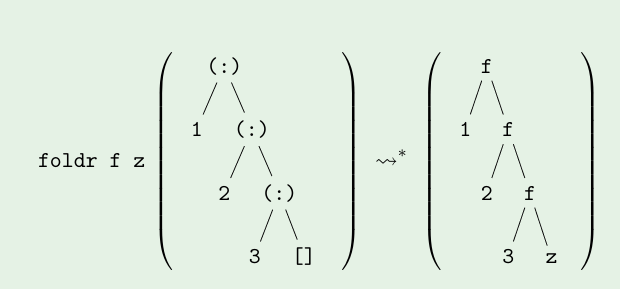
\includegraphics[width=\linewidth]{assets/foldr_grafico.png}
    \end{minipage}%
    \begin{minipage}[b]{0.5\textwidth}
        \centering
        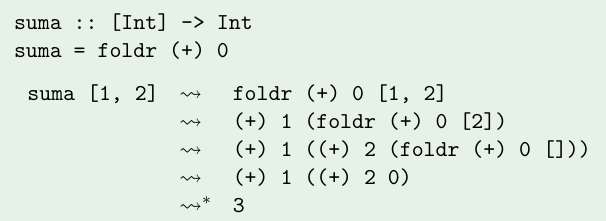
\includegraphics[width=\linewidth]{assets/suma_foldr.png}
    \end{minipage}
\end{figure}
Una función f está dada por recursión estructural sí: 
\begin{itemize}
    \item El caso base devuelve un valor fijo z.
    \item El caso recursivo es una función de x y (g xs)
    \item Se trabaja solamente con la cabeza de la lista.
    \item Se hace recursión sobre la cola pero no se tiene acceso a ella, sino al llamado recursivo.  Es decir, el caso recursivo no usa xs. 
    \item La recursión es la clásica, va desde derecha a izquierda. La R de foldr es de Right. 
\end{itemize}
Su estructura formal es la siguiente 
\begin{lstlisting}
    g [] = <caso base> -> valor 
    g (x:xs) = <caso recursivo> -> función cabeza de la lista y resultado de la recursión.
\end{lstlisting}
Por lo tanto foldr se define como
\begin{lstlisting}
    foldr :: (a -> (b -> b)) -> b -> [a] -> b 
    foldr f z [] = <
    foldr f z (x:xs) = f x (foldr f z xs)
\end{lstlisting}
\textbf{Importantísimo}: El tipado de foldr es $ Foldable \ t \implies (a \rightarrow b \rightarrow b) \rightarrow b \rightarrow t a \rightarrow b $
\begin{itemize}
    \item a = Es el elemento que tenemos actualmente en la recursión.
    \item b = Es cualquier tipo que nos permita acumular. Puede ser una tupla, un número, lo que sea. Pero en cada paso recursivo hay que llenar eso. El caso base tiene que cumplir este tipo b.
    \item Véase \hyperref[subsec:foldr_ejercicios]{\underline{\textbf{anexo}}} para ver ejemplos usando foldr.
\end{itemize}
¿Qué es lo que produce foldr (:) []? Es una identidad sobre listas porque haría recursión sobre una lista vacía. \\
¿Qué es lo que hace la siguiente función foldr? $ foldr(\backslash x \ r \rightarrow x) \ 0 \ [1, 2]$ 
\begin{itemize}
    \item Toma la lista y hace recursión. Empieza con el 2, ejecuta la función y devuelve 2. Hace el paso recursivo.
    \item Toma la lista y hace recursión. Ahora sigue con el 1, recibe 1 y la salida es 1. 
    \item Esta función agarra el primer elemento de una lista, sería el head.
\end{itemize}
\textbf{IMPORTANTÍSIMO}: Se pueden recorrer dos listas, tres listas, las que quieras a la vez con Foldr. La recursion se hace sobre una sola, pero las n-1 listas las enviarías por argumento en cada paso recursivo. Véase \hyperref[subsec:foldr_armar_pares]{\textbf{\underline{anexo}}} para ver ver el árbol de recursión y un ejemplo práctico. 
\textbf{Importante}: Foldr puede trabajar con listas infinitas. \\
Véase \hyperref[subsec:foldr_ex]{\textbf{\underline{anexo}}} para ver ejemplos de Foldr. \\
\subsection*{Recursión que \textbf{no} es estructural}
\begin{lstlisting}
    ssort :: Ord a => [a] -> [a]
    ssort [] = []
    ssort (x:xs) = minimo (x:xs) : ssort(sacarMinimo(x:xs))
\end{lstlisting}
No es estructural pues se esta usando xs para el llamado de minimo(x:xs) y no solamente en el llamado recursivo de ssort.
\subsection*{Iteración (foldl)}
Se la conoce como Plegado a la Izquierda porque va resolviendo inmediatamente de izquierda a derecha hasta que termine el proceso. \\
\begin{figure}[h]
    \centering
    \begin{minipage}[b]{0.5\textwidth}
        \centering
        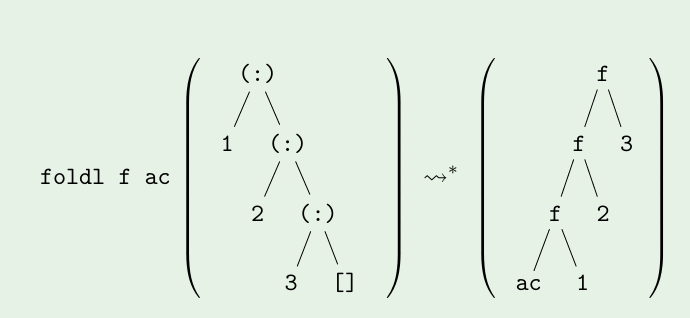
\includegraphics[width=\linewidth]{assets/foldl_grafico.png}
    \end{minipage}%
    \begin{minipage}[b]{0.5\textwidth}
        \centering
        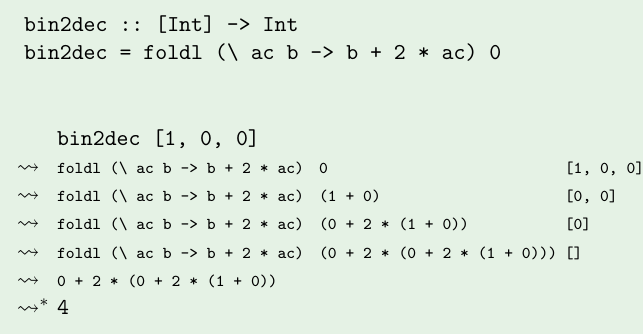
\includegraphics[width=\linewidth]{assets/bin2dec_foldl.png}
    \end{minipage}
\end{figure}
Este tipo de recursión es más que recursión una iteración, en este caso empezamos yendo desde el primer valor hasta el último. \\
En este enfoque voy modificando una solución parcial. \\
Por lo tanto foldl se define como
\begin{lstlisting}
    foldl :: (b -> a -> b) -> b -> [a] -> b 
    foldl f ac [] = ac
    foldl f ac (x:xs) = foldl f (f ac x) xs
\end{lstlisting}
¿Qué es lo que sucede en el siguiente ejemplo? \\
\begin{lstlisting}
    foldl (\x y -> 1) 0 unos
    foldl f (f 0 1) unos
    foldl f(f(f 0 1) 1) unos
\end{lstlisting}
Esto es in-realizable con foldl. Es decir, foldl no puede manejar listas infinitas. \\
\textbf{Importantísimo}: El tipado de foldl es $ Foldable \ t  \implies (b \rightarrow a \rightarrow b) \rightarrow b \rightarrow t a \rightarrow b $
\begin{itemize}
    \item b = Es cualquier tipo que nos permita acumular. Puede ser una tupla, un número, lo que sea. Pero en cada paso recursivo hay que llenar eso. El caso base tiene que cumplir este tipo b.
    \item a = Es el elemento que tenemos actualmente en la recursión.
\end{itemize}
Véase \hyperref[subsec:foldl_ejercicios]{\underline{\textbf{anexo}}} para ver ejemplos usando foldl.
\subsection*{¿Por qué foldl es peor que foldr?}
\textbf{foldl}: Procesa la lista de izquierda a derecha, lo que requiere evaluar toda la lista antes de devolver un resultado, lo que no es posible con listas infinitas. \\
\textbf{foldr}: Procesa la lista de derecha a izquierda, permite trabajar de manera perezosa y puede manejar listas infinitas si la función y el valor inicial permiten una evaluación parcial o completa sin necesidad de procesar todos los elementos.
\subsection*{Recursión Primitiva (recr)}
No existe en Haskell. Es una manera de nosotros podemos tener las mismas ventajas de foldr pero en este caso, la recursión primitiva nos permite utilizar la cola de la lista 
\begin{itemize}
    \item Se trabaja solamente con la cabeza de la lista y la cola.
    \item Se hace recursión sobre la cola.
\end{itemize}
Su estructura forma les la siguiente 
\begin{lstlisting}
    g [] = b
    g (x:xs) = f x xs (g xs)
\end{lstlisting}
Por lo tanto recr se define como 
\begin{lstlisting}
    recr :: (a -> [a] -> b ->b) -> b -> [a] -> b 
    recr f z [] = z
    recr f z (x:xs) = f x xs (recr f z xs)
\end{lstlisting}
\section*{Tipos}
Existen diferentes maneras de definir tipos. Esto es según sea el objetivo.
Definimos tipos con la palabra \textbf{data} + Nombre = Tipo1 | Tipo2 | Tipo 3 \\
Si hacemos en GHCI $:t Tipo1$ saldrá que es de tipo Nombre. \\
\textbf{Nota}: $|$ indica que a continuación hay otro tipo.
\subsection*{Tipos Comunes}
Son no recursivos, ej: $data Dia = Lu | Ma | Mi | Mie | Ju | Vi | Sa | Do $ \\
Lu, Ma, Mi, ... son constructores del tipo dia. \\
Los argumentos podrán ser recibidos diciendo qué tipo se espera, y usamos pattern matching para utilizarlos.
\begin{lstlisting}
    EsLunes :: Dia -> Bool
    EsLunes Lu = True 
    EsLunes _ = False 

    EsFinDeSemana :: Dia -> Bool
    EsFinDeSemana Sa = True 
    EsFinDeSemana Do = True 
    EsFinDeSemana _ = False 
\end{lstlisting}
\subsection*{Tipos con Funciones}
Los tipos también pueden tener tipos que necesiten argumentos. Difieren en la info que devuelven. \\
Ej.: data Persona = LaPersona String String Int \\
\textbf{Importante}
\begin{itemize}
    \item Si evaluamos $:t LaPersona$ sin enviar los argumentos retornará $LaPersona :: String -> String -> Int$. 
    \item Si evaluamos $:t LaPersona "T", "H", 23$ enviando los argumentos retornará que LaPersona es de tipo Persona
\end{itemize}
\begin{lstlisting}
    Edad :: Persona -> Int 
    Edad (LaPersona n a e) = e

    Cumpleaños :: Persona -> Persona 
    Cumpleaños (LaPersona n a e) = LaPersona n a (e+1)
\end{lstlisting}
\textbf{Importante}: Nótese que estamos devolviendo \textbf{una nueva persona}. En programación funcional no existe el concepto de "modificar" algo, sino crear algo nuevo con lo anterior y cambiarle algo.
\subsection*{Tipos Recursivos}
Cuando tengo tipos recursivos, las funciones que los usen deben manejar casos bases y la recursión \\
Ej.: data Nat = Zero | Succ Nat \\
\subsection*{Tipos Polimórficos} 
Al igual que las funciones, podemos definir que los tipos tengan constructores de un tipo específico.
\begin{lstlisting}
    data List a = Vacia | Const a (List a)
\end{lstlisting}
\subsection*{Importante en Tipos}
No se puede repetir un mismo constructor para un mismo tipo. \\
Es decir
\begin{lstlisting}
    data List = Vacia | Cons Int ListI 
    data List a = Vacia | Cost a (List a)

    Error. No puede estar Vacia como constructor de dos tipos diferentes.
\end{lstlisting}

\section*{Listas}
\begin{itemize}
    \item Por extensión: Es dar la lista implícita escribiendo todos sus elementos. Ej. [1, 2, 3]
    \item Secuencias: Progresiones aritméticas en un rango particular. Ej.: [3..7] es la lista que tiene los números del 3 al 7.
    \item Por compresión: Se definen de la siguiente manera [expresion | selectores, condiciones]. Ej.: [(x,y) | x <- [0..5], y <- [0..3], x+y==4] es la lista de pares que tienen elementos de x e y que dan menos que 4
\end{itemize}
\section*{Estructuras Recursivas sobre Otras Estructuras de Datos}
¿Cómo podemos plantear la estructura de un foldr para un árbol binario o cualquier estructura plegable que no sea una lista? \\
Lo primero que podemos intuir es que en las listas, solo hay una recursión, sobre la lista propiamente pero en un Árbol Binario tenemos dos caminos: rama izquierda y rama derecha. Esto quiere decirque de alguna manera, tenemos que capturar 2 recursiones.
\begin{itemize}
    \item Planteamos varios problemas acerca de esa estructura de datos y vemos qué patrones hay en común. 
    \item Las cosas que sean diferentes, las pasamos por parámetros. 
\end{itemize}
Por ejemplo, sean estas operaciones de un árbol binario 
\begin{lstlisting}
    nodos :: AB -> Int 
    nodos Nil = 0
    nodos (Bin i r d) = nodos i + 1 + nodos d 

    preorder :: AB -> [a]
    preorder Nil = []
    preorder (Bin i r d) = [r] ++ preorder i ++ preorder d
\end{lstlisting}
Podemos observar que cambia lo siguiente 
\begin{itemize}
    \item Tipos de salida: En el primer ejemplo devolvemos un int, en el segundo una lista de a. La lista de a sería el tipo que tenga el AB. 
    \item Caso base: En uno es [] y en otro 0. Por lo tanto tenemos que admitir un tipo b para el caso base. El caso base es del mismo tipo que el tipo de salida \textbf{siempre}.
    \item Función que realiza: En uno hace sumas, en el otro hace concatenaciones. 
\end{itemize}
¿Cómo podríamos escribir las funciones anteriormente mencionadas de manera anónima? 
\begin{lstlisting}
    nodos: (\ri r rd -> ri + 1 + rd)(nodos i) r (nodos d)
    preorder: (\ri r rd -> [r] ++ ri ++ rd) (preorder i) r (preorder d)
\end{lstlisting}
Recordemos la firma de foldr: $Foldable \ t \ \implies \ (a \ \rightarrow \ b \ \rightarrow \ b) \ \rightarrow \ b \ \rightarrow \ t \ a \ \rightarrow \ b$ \\
Donde b era el caso base / recursivo y a el elemento actual, acá tenemos dos. \\
Recordemos la estructura del tipo AB: AB a = Nil | Bin (AB a) a (AB a) \\
Entonces nuestra función foldAB va a tener que estar preparado para recibir ambos (AB a) y a.
foldAB :: (b $\rightarrow$ a $\rightarrow$ b $\rightarrow$ b) $\rightarrow$ b $\rightarrow$ AB a $\rightarrow$ b donde :t Bin: (AB a) $\rightarrow$ a $\rightarrow$ (AB) a $\rightarrow$ AB a donde 
\begin{itemize}
    \item $(b \rightarrow a \rightarrow b \rightarrow b)$
    \begin{itemize}
        \item la primera b: recursión rama izquierda
        \item la a: la raíz 
        \item la segunda b: recursión rama derecha 
        \item la tercera b: el resultado del proceso.
    \end{itemize}
    \item b: el resultado.
    \item AB a: la entrada 
    \item b: el resultado.
\end{itemize}
Es súper importante entender que la firma de la función que acepta foldAB está prácticamente atada al tipo de la estructura de dato.
\section*{Validación y Verificación de Programas}
\begin{itemize}
    \item Trabajaremos con estructuras de datos \textbf{finitas}. Más técnicamente, con tipos de datos \textbf{inductivos}.
    \item Trabajamos con \textbf{funciones totales}
    \begin{itemize}
        \item Las ecuaciones deben cubrir todos los casos posibles.
        \item La recursión siempre termina.
    \end{itemize} 
    \item El programa \textbf{no depende del orden} de las ecuaciones. 
\end{itemize}
\section*{Principio de Reemplazo}
Sea $e1 = e2$ una ecuación del programa. Las siguientes operaciones preservan la igualdad de expresiones.
\begin{itemize}
    \item Reemplazar \textbf{cualquier instancia} de e1 por e2.
    \item Reemplazar \textbf{cualquier instancia} de e2 por e1.
\end{itemize}
\textbf{Importante}: Si una igualdad se puede demostrar usando sólo el principio de reemplazo, decimos que la igualdad vale \textbf{por definición}.
\[\begin{minipage}[b]{0.9\textwidth}
    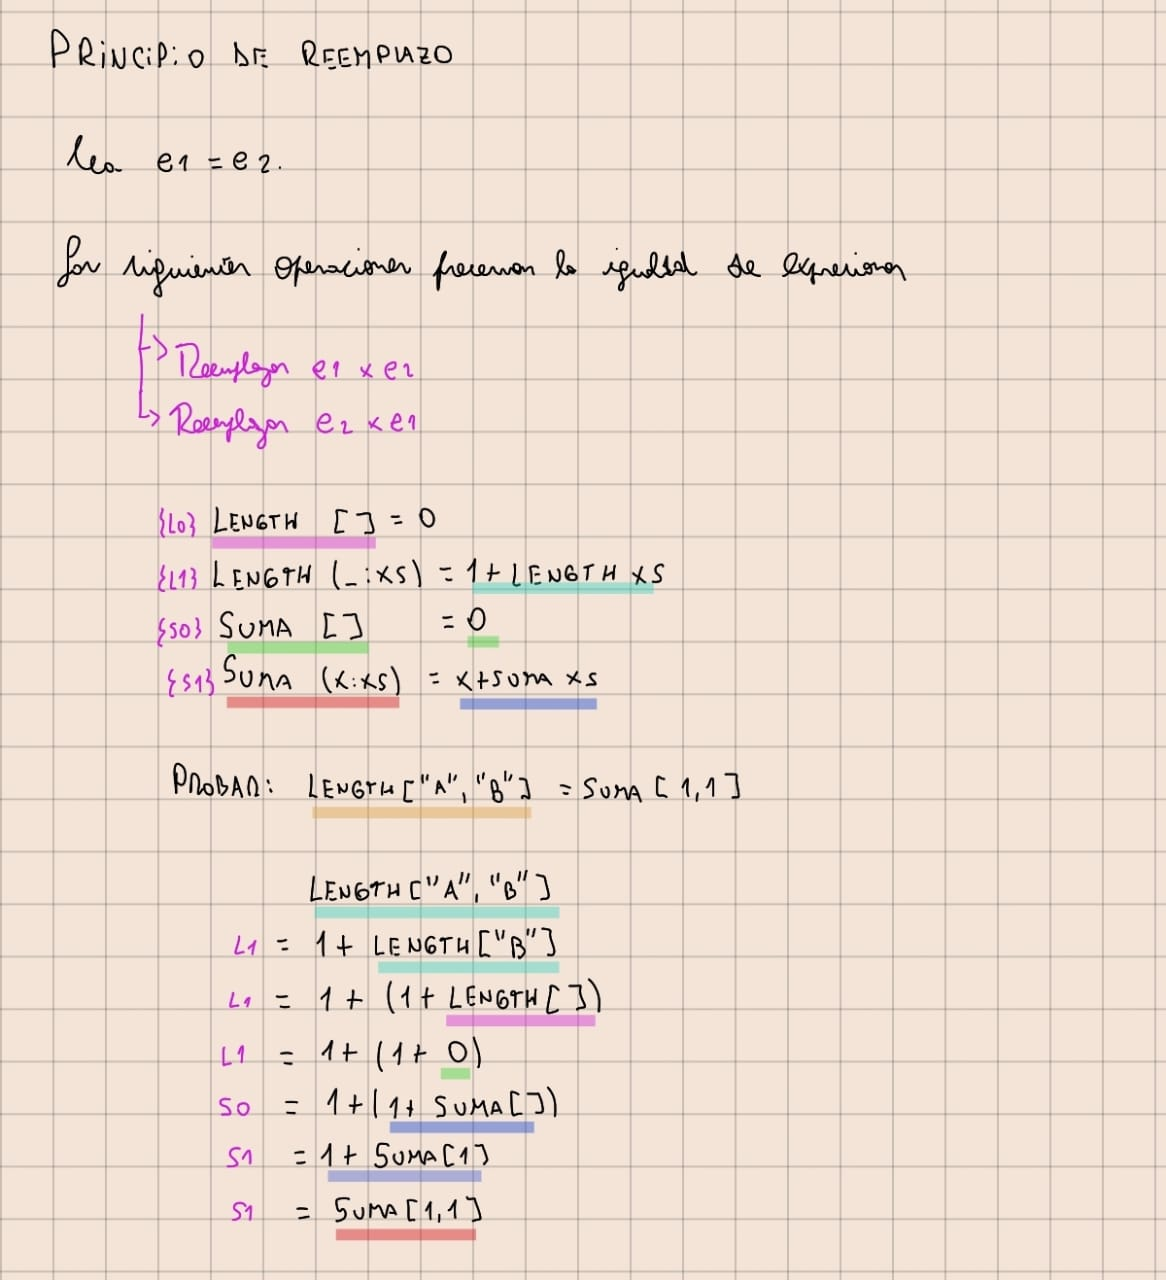
\includegraphics[width=\linewidth]{assets/principio_reemplazo_dibujo.jpg}
\end{minipage}\]
\section*{Inducción Estructural}
Cada tipo de datos tiene su propio principio de inducción. \\
\textbf{Importante}: El . acá cumple el rol del () en el $\forall$ es decir $\forall x :: Bool . \mathcal{P} \equiv (\forall x :: Bool)(\mathcal{P}) $ y el $::$ cumple el rol de \textbf{es del tipo...}
\subsection*{Inducción sobre booleanos}
Si $\mathcal{P}(True)$ y $\mathcal{P}(False)$ entonces $\forall x :: Bool \ \mathcal{P} (x)$ 
\[\begin{minipage}[b]{0.7\textwidth}
    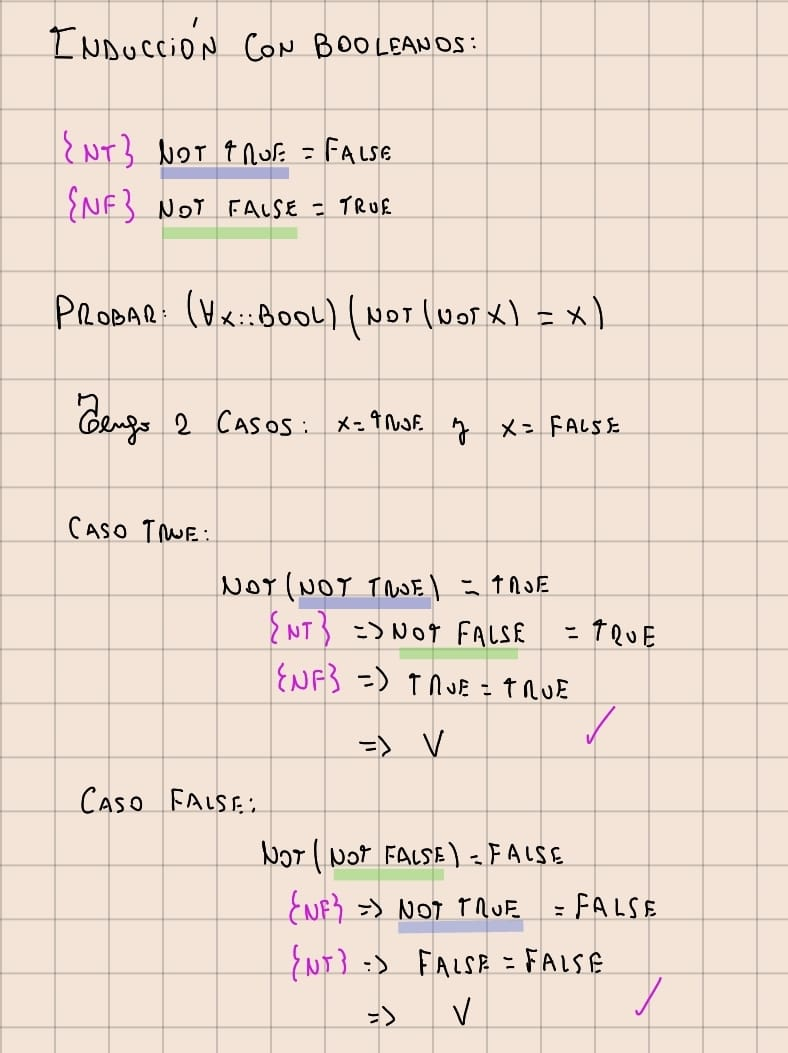
\includegraphics[width=\linewidth]{assets/induccion_booleanos_dibujo.jpg}
\end{minipage}\]
\subsection*{Inducción sobre pares}
Si $(\forall x :: a)(\forall y :: b)(\mathcal{P}(x, y))$ entonces $\forall p :: (a, b) \mathcal{P}(p)$
\[\begin{minipage}[b]{0.7\textwidth}
    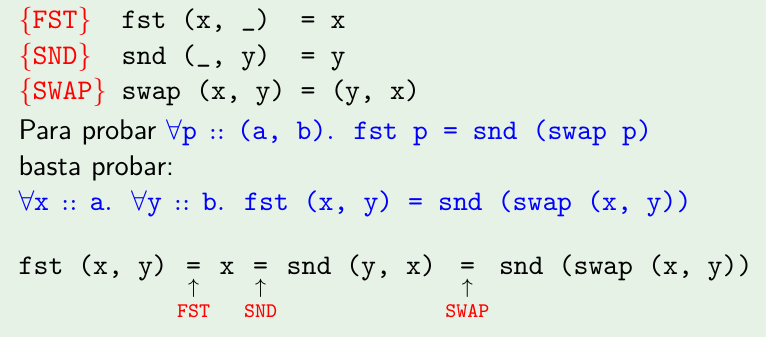
\includegraphics[width=\linewidth]{assets/induccion_pares.png}
\end{minipage}\]
\[\begin{minipage}[b]{0.7\textwidth}
    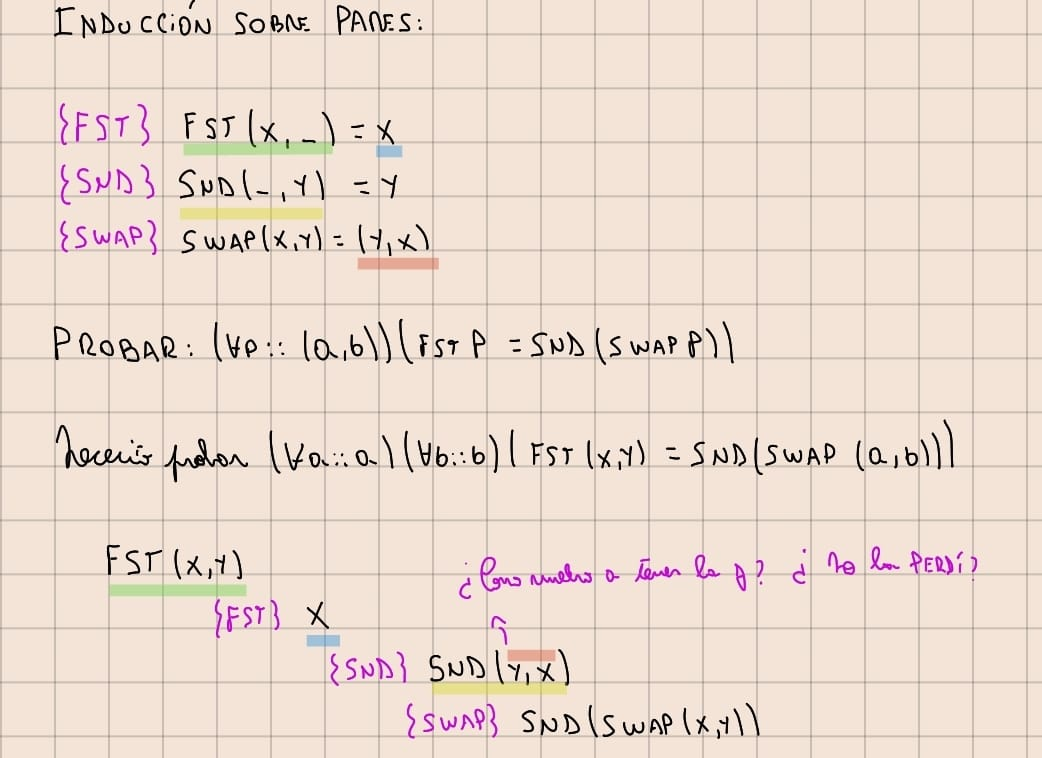
\includegraphics[width=\linewidth]{assets/induccion_pares_dibujo.jpg}
\end{minipage}\]
\subsection*{Inducción sobre naturales}
Si $\mathcal{P}(Zero)$ y $(\forall n :: Nat)(\mathcal{P}(n) \implies \mathcal{P}(Suc \ n))$ entonces $(\forall n :: Nat)(\mathcal{P}(n))$ donde 
\begin{itemize}
    \item $\mathcal{P}(n)$: Hipótesis Inductiva.
    \item $\mathcal{P}(Suc \ n)$: Tesis Inductiva.
\end{itemize}
\[\begin{minipage}[b]{0.7\textwidth}
    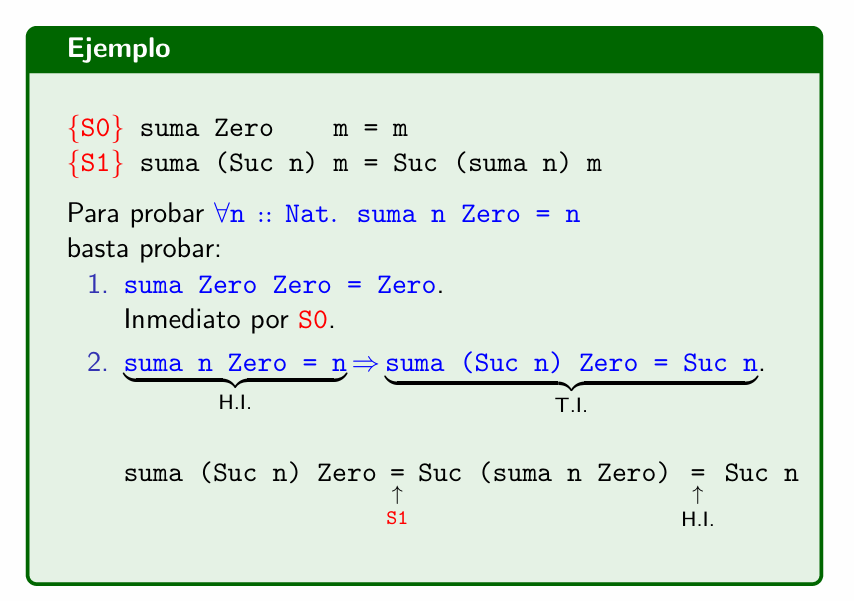
\includegraphics[width=\linewidth]{assets/induccion_naturales.png}
\end{minipage}\]
\[\begin{minipage}[b]{0.7\textwidth}
    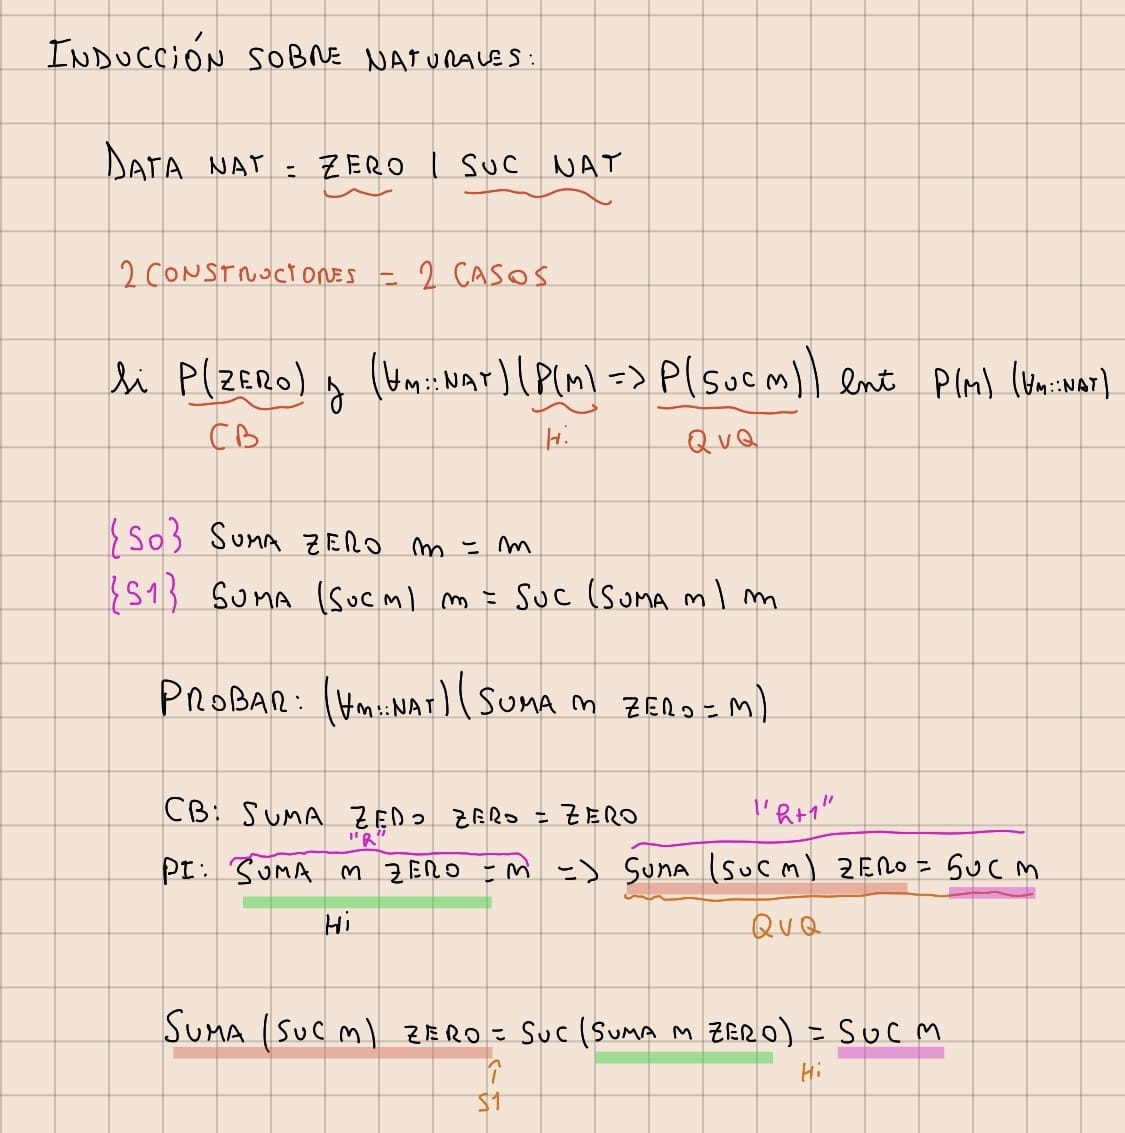
\includegraphics[width=\linewidth]{assets/induccion_naturales_dibujo.jpg}
\end{minipage}\]
\subsection*{Inducción Estructural: Caso General}
Sea $\mathcal{P}$ una propiedad acerca de las expresiones tipo T tal que 
\begin{itemize}
    \item $\mathcal{P}$ vale sobre todos los constructores base de T,
    \item $\mathcal{P}$ vale sobre todos los constructores recursivos de T, asumiendo como hipótesis inductiva que vale para los parámetros de tipo T,
\end{itemize}
entonces $(\forall x :: T)(\mathcal{P}(x))$
\subsection*{Principio de Inducción sobre Listas}
\[\begin{minipage}[b]{0.9\textwidth}
    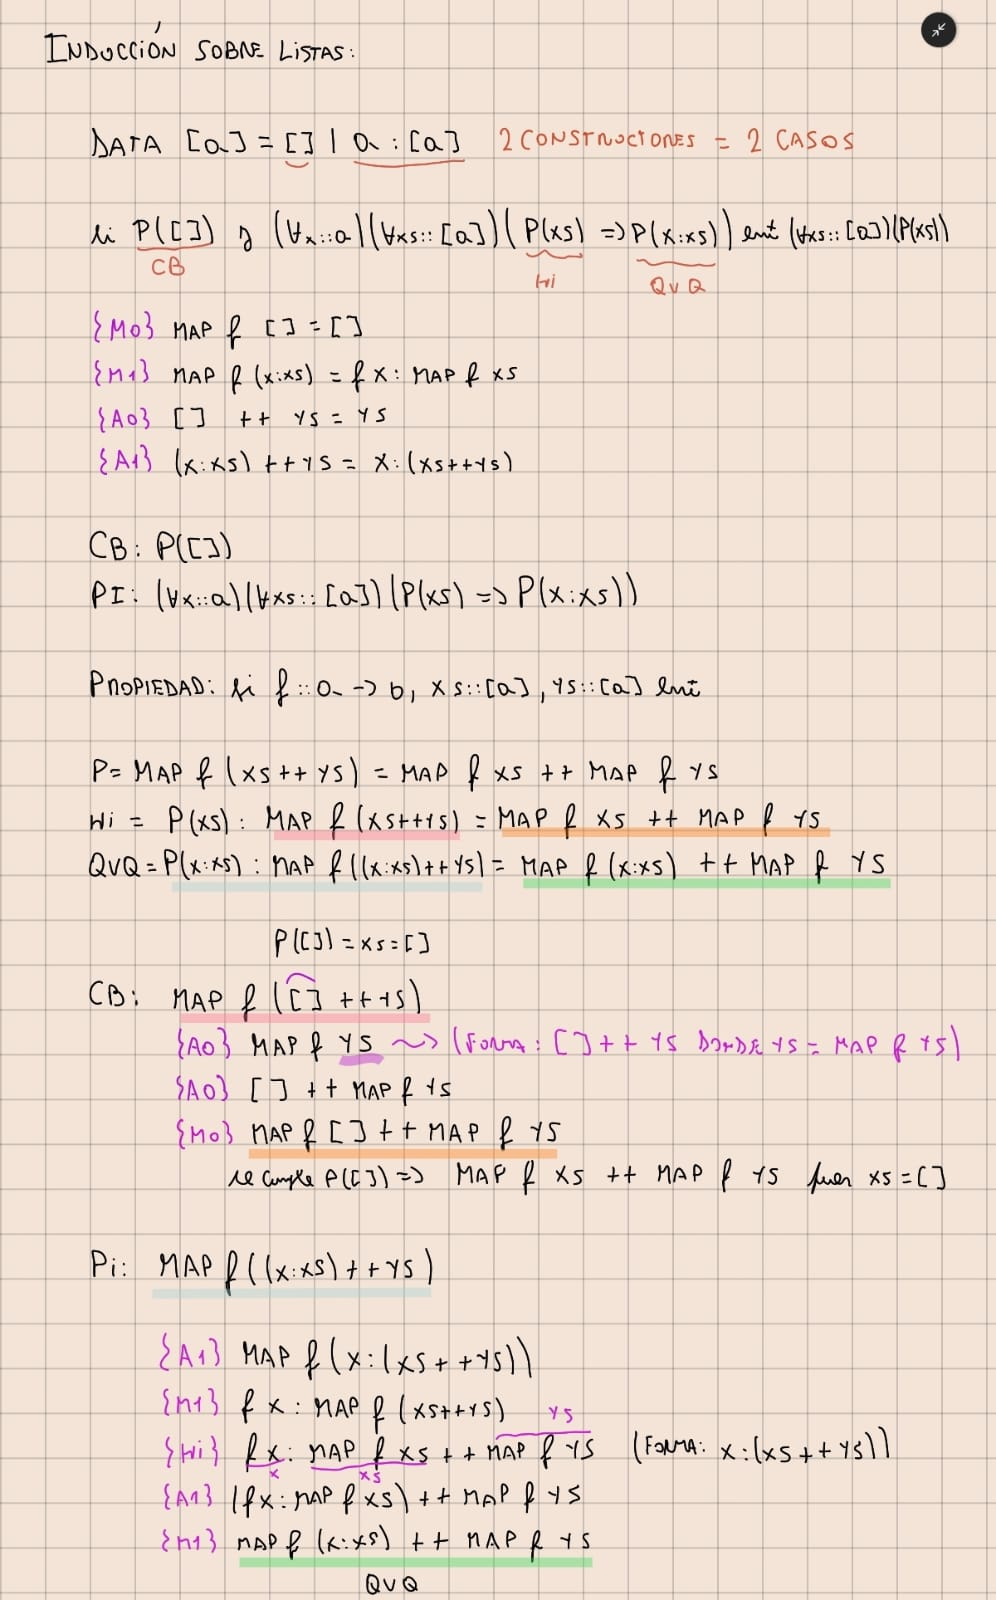
\includegraphics[width=\linewidth]{assets/induccion_listas_dibujo.jpg}
\end{minipage}\]
\subsection*{Principio de Inducción sobre Árboles Binarios}
\[\begin{minipage}[b]{0.7\textwidth}
    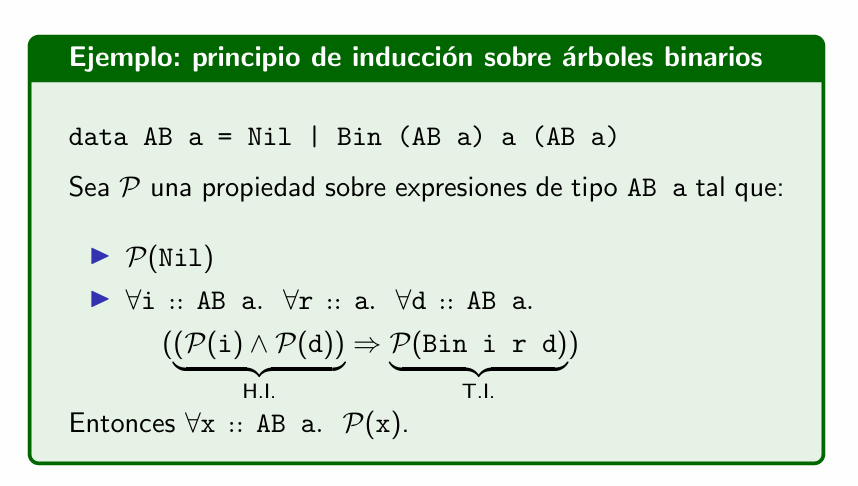
\includegraphics[width=\linewidth]{assets/principio_induccion_ab.png}
\end{minipage}\]
\subsection*{Principio de Inducción sobre Polinomios}
\[\begin{minipage}[b]{0.7\textwidth}
    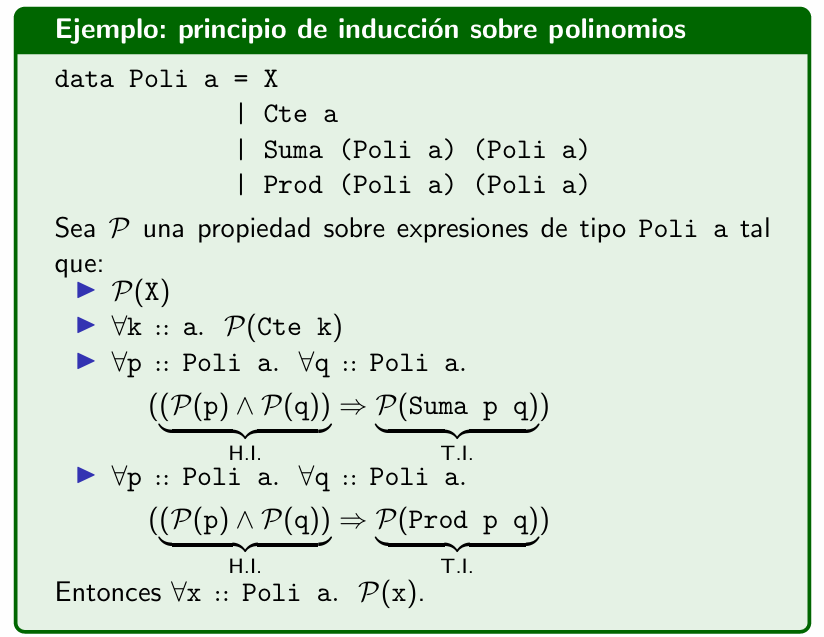
\includegraphics[width=\linewidth]{assets/principio_induccion_polinomios.png}
\end{minipage}\]
\subsection*{Relación entre foldr y foldl}
\textbf{Propiedad}: Si $f::a\rightarrow b \rightarrow b, \ z::b, \ xs::[a]$ entonces foldr f z xs = foldl (flip f) z (reverse xs) \\
\textbf{Lema}: Si $g::b \rightarrow a \rightarrow b, \ z::b, x::a, xs::[a]$ entonces foldl g z (xs ++ [x]) = g (foldl g z xs) xs
\subsection*{Puntos de vista intensional vs extensional}
Sí, es con \textbf{s}. Es intensional. \\
¿Es equivalente mergesort = insertionSort? La realidad es que: hacen lo mismo (llegan al mismo resultado); ordenan algo pero de una manera diferente.
\begin{itemize}
    \item Punto de vista intensional: Dos valores son iguales si están definidos de la misma manera.
    \item Punto de vista extensional: Dos valores son iguales si son indistinguibles al observarlos.
\end{itemize}
Entonces mergesort = insertionSort desde el lado extensional, porque hacen lo mismo pero no son iguales desde el punto de vista intensional. 
\subsection*{Principio de Extensionalidad Funcional}
Sean $f, \ g :: a \rightarrow b$. \\
\textbf{Principio de extensionalidad funcional}: Si $(\forall x :: a)(f \ x  =  g \ x) $ entonces $f=g$ \\
El ppio. de extensionalidad funcional nos dice que si son funciones son iguales entonces son iguales punto a punto donde las evaluemos.
\subsection*{Demostración de Desigualdades}
¿Cómo demostramos que no vale una igualdad e1 = e2 :: A? \\
Entiendo que básicamente hay que encontrar hacer \textbf{ALGO} para demostrar que no son iguales. Este \textbf{ALGO} es una funcionalidad que devuelva algo con uno, y otra cosa con otro. Por lo tanto debería ser del tipo $obs \ a :: A \rightarrow Bool$. \\
Demostrar que \textbf{no} vale la igualdad: $id = swap :: (Int, Int) \rightarrow (Int, Int)$. \\
Esto es fácil de probar porque sabemos que $id$ nos da exactamente lo mismo que envíamos, y swap justamente da vuelta todo. Por lo tanto podemos comparar el primer elemento con id y el primer elemento haciendo el swap. \\
Ej.: $(1, 2) \rightarrow id (1, 2) \rightarrow (1, 2)$ pero $swap (1, 2) = (2, 1)$ y el primer elemento de $id (1, 2) \rightarrow (1, 2)$ es decir, $1 \neq 2$ que arroja el swap. \\
Por lo tanto
\begin{lstlisting}
    Ej: (1, 2)
    obs :: ((Int, Int) -> (Int, Int)) -> Bool 
    obs f = fst (f (1,2)) == 1

    obs id -> True 
    obs swap False
\end{lstlisting}
Nótese que el obs está \textbf{exactamente armado para este caso particular}. Para demostrar que las funciones no hacen lo mismo.
\section*{Isomorfismo de Tipos}
Decimos que dos tipos son isomorfos si podemos pasar de uno al otro aplicando alguna función y al componerlas el resultado arroja la función identidad. 
\begin{lstlisting}
    ("hola", (1, True)) :: (String, (Int, Bool))
    ((True, "hola"), 1) :: ((Bool, String), Int)
    Estos dos tipos son isomorfos porque podemos transformar los valores de un tipo en valores del otro

    f :: (String, (Int, Bool)) -> ((Bool, String), Int)
    f (s, (i, b)) = f((b, s), i)

    g :: ((Bool, String), Int) -> (String, (Int, Bool))
    g ((b, s), i) = f (s, (i, b))

\end{lstlisting}
¡Es básicamente crear una función que reciba los parámetros de otra manera y los mande a la otra función de la otra forma! Una especie de Curry/Uncurry. \\
Con esto se puede demostrar que $g . f = id$ y $f . g = id$ \\
Formalmente, podemos decir que dos tipos de datos A y B son \textbf{isomorfos} si 
\begin{itemize}
    \item Hay una función $f :: A \rightarrow B$ total.
    \item Hay una función $g :: B \rightarrow A$ total 
    \item Se puede demostrar que $g . f = id :: A \rightarrow A$
    \item Se puede demostrar que $f . g = id :: B \rightarrow B$
\end{itemize}
En criollo: Debe existir una función que me mapee de f a g y viceversa. Por último, si hago f(g) o g(f) tienen que dar la identidad. \\
\textbf{Notación}: $A \simeq B$ indican que A y B son isomorfos.
\section*{Intérpretes}
Un intérprete ejecuta programas, no los traduce como si fuese un compilador. 
\subsection*{Sintaxis Concreta}
Se pueden representar programas como cadenas de texto. Es tedioso de interpretar algo así: if $x>0$ then x else -x 
\subsection*{Sintaxis Abstracta}
Podemos representar instrucciones a través de árboles: (Eif (gt (var "x") cte 0)) (var("x")) (neg (var("x")))
\subsection*{Lenguaje de Expresiones Aritméticas}
Veamos como hacer un intérprete que pueda reconozca números y haga sumas. \\
Primero tenemos que definir los tipos de expresiones que vamos a querer reconocer (expresiones) en nuestro intérprete.
\begin{lstlisting}
    data Expr = EConstNum Int 
              | EAdd Expr Expr 
\end{lstlisting}
Nótese que EAdd es un constructor del tipo Expr recursivo que en algún momento llegará al caso base de EConstNum que devuelve un Int. \\
¿Es posible comparar los resultados de las Expr desde una manera de igualdad? ¡No! Los tipos no aceptan \textbf{ningún tipo de operación} a menos que lo indiquemos. Si queremos que estos tipos puedan compararse de la siguiente forma $n_{1} = n_{2}$ tenemos que configurar \textbf{deriving (EQ)} donde EQ es una clase. 
\begin{lstlisting}
    data Expr = EConstNum Int 
              | EAdd Expr Expr 
              deriving Eq
\end{lstlisting}
¿Es posible mostrar el resultado en consola de las operaciones que hagamos? ¡No! Los tipos no aceptan \textbf{ningún tipo de operación} a menos que lo indiquemos. Si queremos que el resultado pueda mostrarse en consola de alguna manera específica tenemos que hacer una instancia de Show. 
\begin{lstlisting}
    instance Show Expr where
    show = showExpr
      where 
        showExpr :: Expr -> String 
        showExpr (EConstNum n) = show n
        showExpr (EAdd e1 e2) = "(" ++ show e1 ++ "+" ++ show e2 ++ ")"
\end{lstlisting}
Bueno, ahora sí. ¿Cómo podemos usar todo esto para computar nuestras expresiones? Necesitamos de alguna manera una función que nos permita enviar expresiones, tomarlas por pattern matching y hacer algo. 
\begin{lstlisting}
    evalExpr :: Expr -> Int
    evalExpr (EConstNum n) = n
    evalExpr (EAdd n m) = evalExpr n + evalExpr m
\end{lstlisting}
Pero ¿cómo lo usamos?. Primero tenemos que llamar a la función enviando la información que nos pide, es decir, algo del tipo Expr. \\
Probemos hacer 1+2, esto en sintáxis concreta sería algo como: $evalExpr \ (EAdd \ (EConstNum \ 1) \ (EConstNum \ 2))$. ¡Nótese que estamos utilizando los constructores del tipo! \\
Entonces, el resultado es: $ghci> \ evalExpr \ (EAdd \ (EConstNum \ 1) \ (EConstNum \ 2)) \implies 3$
\subsection*{Nuestro Lenguaje de Expresiones Aritméticas con Booleanos}
Queremos agregarle booleanos a nuestro lenguaje. ¿Qué debemos hacer? Lo primero es lo primero, tenemos que ver si debemos refactorizar algo o simplemente extender. Como hasta ahora hicimos solamente cosas de números raramente vamos a tener que refactorizar algo aunque eso está por verse. \\
Por lo tanto lo primero que debemos hacer es aceptar que el booleano sea un constructor del tipo Expr
\begin{lstlisting}
    data Expr =   EConstNum Int 
                | EConstBool Bool 
                | EAdd Expr Expr 
\end{lstlisting}
Entonces ahora podemos extender la clase Show 
\begin{lstlisting}
        ... mismo antes
        showExpr (EConstBool b) = show b
\end{lstlisting}
Por último, podemos aceptar evaluar la expresión de booleano (que sería un caso base) ante eventuales operaciones de este tipo. \\
\begin{lstlisting}
    evalExpr :: Expr -> Int
    evalExpr (EConstNum n) = n
    evalExpr (EConstBool b) = b
    evalExpr (EAdd n m) = evalExpr n + evalExpr m
\end{lstlisting}
¿Cuál es el problema que estamos viendo? El problema es que ahora evalExpr \textbf{no} solo devuelve Int sino que Bool. Por esto, podemos crear un nuevo tipo que sean los tipos de salida de nuestras expresiones. \\
\begin{lstlisting}
    data Val = VN Int | VB Bool  deriving Eq
\end{lstlisting}
Luego, 
\begin{lstlisting}
    evalExpr :: Expr -> Val
    evalExpr (EConstNum n) = n
    evalExpr (EConstBool b) = b
    evalExpr (EAdd n m) = evalExpr n + evalExpr m
\end{lstlisting}
Pero ahora hay otro problema: \textbf{evalExpr n y evalExpr m devuelven un tipo Val, el tipo Val es un Int | Bool}. Veamos para qué tipos está permitida la suma infija (Num a => a -> a -> a). Por lo tanto, \textbf{ahora que estamos usando Val no podemos usar la suma porque Val no necesariamente es un número, también puede ser un booleano}. Así que como nosotros sabemos que \textbf{vamos a usar el +} cuando tenemos números hay que hacer una función específica para ese tipo. \\
Creamos entonces, una función que vamos a llamar para que nos devuelva una nueva instancia del tipo Val que haga las sumas correspondientes
\begin{lstlisting}
    addVal :: Val -> Val -> Val 
    addVal (VN n) (VN m) = VN (n+m)
    addVal _ _ = error "Algún sumando no es numérico"
\end{lstlisting}
Por lo tanto, reemplazamos + con addVal 
\begin{lstlisting}
    evalExpr :: Expr -> Val
    evalExpr (EConstNum n)  = VN n
    evalExpr (EConstBool b) = VB b
    evalExpr (EAdd n m) = addVal (evalExpr n) (evalExpr m)
\end{lstlisting}
¿Qué falta ahora? Configurar el show de nuestra nueva clase Val porque evalExpr nos devuelve algo de tipo Val y todavía no definimos cómo mostrarlo. 
\begin{lstlisting}
    instance Show Val where 
    show = showVal 
        where 
            showVal :: Val -> String 
            showVal (VN n) = show n
            showVal (VB b) = show b
\end{lstlisting}
Por último, ejecutamos igual que antes y funcionará todo: $evalExpr \ (EAdd \ (EConstNum \ 1) \ (EConstNum \ 2)) \rightarrow 3$
\subsection*{Nuestro Lenguaje de Expresiones con Definiciones en el Ambiente}
Queremos aceptar expresiones del tipo $let \ x=3 \ in \ (let \ y = x+x \ in \ 1+y)$ \\
Recordemos que en Haskell, un let define una variable en un environment para que la podamos utilizar. Si nosotros llegaramos a mencionar una variable y no está definida da error. \\
Sabiendo esto, necesitamos dos procedimientos: definir una variable con un valor, y una función que dada una variable me de su valor. \\
Extendamos nuestro tipo de Expr 
\begin{lstlisting}
    type Id = String 
    data Expr = EConstNum Int 
                | EConstBool Bool 
                | EAdd Expr Expr  
                | ELet Id Expr Expr 
                | EVar Id
\end{lstlisting}
\textbf{Nota}: Id es básicamente la forma que vamos a identificar las variables, en este caso con un String. Ej. "x" \\
¿Qué es lo que tenemos que refactorizar? Tenemos que aceptar los casos de EVar y ELet en nuestro evalExpr por lo tanto 
\begin{lstlisting}
    evalExpr :: Expr -> Val
    evalExpr (EConstNum n)  = VN n
    evalExpr (EConstBool b) = VB b
    evalExpr (ELet x e1 e2) = ?
    evalExpr (EVar x) = ?
    evalExpr (EAdd n m) = addVal (evalExpr n) (evalExpr m)
\end{lstlisting}
¿Cúal es el problema de esto? ¡No tenemos en el environment donde queremos almacenar la definición de la variable x! \\
\textbf{Importante}: Recordar que el Environment de Haskell inicialmente vamos a enviarlo vacío. Si llegase a haber una acción sobre él, devolvemos una instancia nueva. \\
Ej.: Si tenía x = 2 y ahora quiero agregar z = 4, voy a tener lo anterior + z = 4 en un nuevo ambiente. Sería una especie de asegura de especificación. \\
Por lo tanto, definamos \textbf{de qué manera} vamos a usar el Environment. 
\begin{lstlisting}
    
    data Env a = EE [(Id, a)]

    emptyEnv :: Env a
    emptyEnv = EE []

    lookupEnv :: Env a -> Id -> a
    lookupEnv (EE e) x = 
    case lookup x e of
        Just y  -> y
        Nothing -> error ("La variable " ++ x ++ " no está definida.")

    extendEnv :: Env a -> Id -> a -> Env a
    extendEnv (EE e) x a = EE ((x, a) : e)

    data Val = VN Int | VB Bool | VS String deriving Eq -> Agregamos VS String (para el ID)

    instance Show Val where 
    show = showVal 
        where 
            showVal :: Val -> String 
            showVal (VN n) = show n
            showVal (VB b) = show b
            showVal (VS s) = show s -> Agregamos
\end{lstlisting}
Ahora sí, extendamos nuestro evalExpr 
\begin{lstlisting}
    evalExpr :: Expr -> Env Val -> Val
    evalExpr (EConstNum n) _  = VN n
    evalExpr (EConstBool b) _ = VB b
    evalExpr (EAdd n m) env = addVal (evalExpr n env) (evalExpr m env)
    evalExpr (EVar x) env = lookupEnv env x
    evalExpr (ELet x e1 e2) env = ?
\end{lstlisting}
¿Cómo definimos x con la expresión 1 y la expresión 2? \\
Recordemos nuevamente, que acá tenemos que ir pisando el environment, que x es una expresión y en el environment tenemos que guardar su \textbf{valor} por lo tanto no hay que olvidarnos de obtener el valor de x.
\begin{lstlisting}
    evalExpr (ELet x e1 e2) env = 
                let v = evalExpr e1 env 
                    env' = extendEnv env x v 
                in evalExpr e2 env'
\end{lstlisting}
Luego, agregamos el show a la aplicación del let y el var 
\begin{lstlisting}
    ...lo anterior
    showExpr (ELet x e1 e2) = "let " ++ x ++ " = " ++ show e1 ++ " in " ++ show e2
    showExpr (EVar x) = x
\end{lstlisting}
Ahora, ejecutemos alguna instrucción que haya funcionado antes \\ 
$evalExpr \ (EAdd \ (EConstNum \ 1) \ (EConstNum \ 2)) \ emptyEnv \rightarrow 3$ \\
Probemos ahora sí ejecutar expresiones del tipo let y var. Definamos una variable x = 3, hagamos y = 4 y luego x + y 
\begin{itemize}
    \item Sintaxis
    \begin{itemize}
        \item Input: (ELet $"x"$ (EConstNum 3) (ELet $"y"$ (EConstNum 4) (EAdd (EVar $"x"$) (EVar $"y"$))))
        \item Output Esperado: let x = 3 in let y = 4 in (x+y)
    \end{itemize}
    \item Código 
    \begin{itemize}
        \item Input: evalExpr (ELet $"x"$ (EConstNum 3) (ELet $"y"$ (EConstNum 4) (EAdd (EVar $"x"$) (EVar $"y"$)))) emptyEnv
        \item Output: 7
    \end{itemize}
\end{itemize}
\subsection*{Simulando un Lenguaje Imperativo con nuestro Intérprete}
¿Qué es lo que tiene un lenguaje imperativo que no tiene un lenguaje funcional? la asignación. \\
La asignación en un lenguaje imperativo se hace comúmente de la siguiente forma 
\begin{itemize}
    \item El nombre de la variable se busca su address en memoria. 
    \item Se hace una escritura sobre ese address con un nuevo valor manteniendo el mismo nombre.
\end{itemize}
Entonces de alguna manera necesitamos simular una memoria. Para eso definamos el tipo y las funciones que necesitamos (los dió la catedra). 
\begin{lstlisting}
    module Memory(Addr, Mem, emptyMem, freeAddress, load, store) where

    type Addr = Int
    data Mem a = MM [(Addr, a)]

    instance Show (Mem a) where
    show (MM _) = "<memoria>"

    emptyMem :: Mem a
    emptyMem = MM []

    freeAddress :: Mem a -> Addr
    freeAddress (MM []) = 0
    freeAddress (MM xs) = maximum (map fst xs) + 1

    load :: Mem a -> Addr -> a
    load (MM xs) a =
    case lookup a xs of
        Just b  -> b
        Nothing -> error "La dirección de memoria no está."

    store :: Mem a -> Addr -> a -> Mem a
    store (MM xs) a b = MM ((a, b) : xs)

\end{lstlisting}
Luego, modificamos las acciones que pueden tener nuestras expresiones en un lenguaje imperativo: asignar un valor nuevo a una variable y ejecutar una secuencia de expresiones  
\begin{lstlisting}
    type Id = String 
    data Expr = EConstNum Int 
                | EConstBool Bool 
                | EAdd Expr Expr  
                | ELet Id Expr Expr 
                | EVar Id
                | EAssignID Expr 
                | ESeq Expr Expr 
\end{lstlisting}
Entonces ahora sí ¿qué cambia de evalExpr? 
\begin{itemize}
    \item Ya no recibimos el valor por una Env sino que ahora recibimos un address.
    \item El valor de un address particular está atado a la memoria y depende de esa memoria. 
\end{itemize}
\begin{lstlisting}
    evalExpr :: Expr -> Env Addr -> Mem Val -> (Val, Mem Val)
    evalExpr (EVar x) env mem = (load mem(lookupEnv x), mem)
    evalExpr (EAdd e1 e2) env mem =
            let (v1, mem') = evalExpr e1 env mem 
            let (v2, mem') = evalExpr e2 env mem'
            in (addVal v1 v2, mem'')
    evalExpr (ELet x e1 e2) env mem = 
            let addr = freeAddr mem 
            (val, mem') = evalExpr e1 env mem 
                mem'' = store mem' addr v 
            in evalExpr e2 env' mem''
    evalExpr (EAssign x expr) env mem = 
            let addr = lookupEnv env x 
            (v, mem') = evalExpr e env mem 
                mem'' = store mem' addr v 
            in (v, mem'')
        
    evalExpr (ESeq e1 e2) env mem = 
        let (v1, mem') = evalExpr e1 env mem 
        in eval e2 env mem'
\end{lstlisting}
\subsection*{Agregando los condicionales a nuestro intérprete}
\begin{lstlisting}
    evalExpr (EIf c t e) env mem = 
        case eval c env mem of 
            (VB b, m) -> evalExpr (if b then t else e) env m
            (VN n, m) -> error "Cond no bool"
\end{lstlisting}
\textbf{Nota}: Es posible encontrar este código en la carpeta de teóricas hecho por mí.
\section*{Características Funcionales}
Volvamos a nuestro lenguaje púramente funcional sin memoria ni direcciones. \\
\begin{lstlisting}
    evalExpr :: Expr -> Env Val -> Val
    evalExpr (EConsNum n) _ = h 
    evalExpr (EConsBool b) _ = b
    evalExpr (EAdd e1 e2) _ = evalExpr e1 env 'addVal' evalExpr e2 env
    evalExpr (EVar x) env = lookup env x 
    evalExpr (ELet x e1 e2) env = evalExpr e2 (extendEnv env x (evalExpr x env))
    evalExpr (EIf c t e) env = evalExpr (if isTrue(evalExpr c env) then t else e) env 
        where isTrue (v b x) = x
              isTrue _ = False 
\end{lstlisting}
Prácticamente todos los lengaujes funcionales están basados en el cálculo-$\lambda$ \\
El cálculo-$\lambda$ es un lenguaje que tiene solamente tres constructores. 
\begin{itemize}
    \item EVar Id $ -- x$
    \item ELam Id Expr $-- \backslash x \rightarrow e $
    \item EApp Expr Expr $-- e1 \ e2$
\end{itemize}
Ahora queremos evaluar cosas como $(\backslash x \rightarrow x + x)$ \\
Por lo tanto en nuestro data Val agreguemos el constructor VFunction, y en las expresiones que queremos evaluar agreguemos la composición y las funciones lambda. \\
\begin{lstlisting}
    data Val = VN Int | VB Bool | VFunction Id Expr 

    data Expr = ... 
                | ELan Id expr -- \x -> c 
                | EApp expr expr -- e1(e2)
\end{lstlisting}
Ahora agreguemos el cuerpo de esas operaciones de expresiones 
\begin{lstlisting}
    ...
    evalExpr (ELam x e) env = VFunction x e 
    evalExpr (EApp e1 e2) env = 
        let v1 = evalExpr e1 env 
        let v2 = evalExpr e2 env 
        in case v1 of 
            VFunction x e -> evalExpr e (extendEnv env x v2)
                        _ -> error "aplicando una no funcion"
\end{lstlisting}
\textbf{Importante}: la e es el cuerpo de la función mientras que (extendEnv env x v2) es el pasaje de parámetros a una función lambda. Los parámetros se pasan a través del environment. \\
Con esta implementación tenemos un problema, si queremos hacer lo siguiente 
\begin{lstlisting}
    let suma = \x -> \ y -> x + y in
    let f = suma 5 in 
    let x = 0 in 
        f 3 
\end{lstlisting}
Tenemos el problema que nosotros querríamos que eso sea 8, pues estamos justamente aplicando parcialmente suma enviando un 5 pero esto da 3. ¿Por qué? \\
En Haskell, este comportamiento no sucede (porque ya lo contempla) pero es importante entender \textbf{qué es lo que pasa}. \\
Cuando hacemos let f = suma 5, f es un nombre a la función parcialmente aplicada suma que como primer argumento se le envía 5. \\
Sin embargo, cuando hacemos x = 0 f 3 lo que estamos haciendo es pisar el comportamiento de f diciendo ahora que la x que antes habíamos indicado vía (suma 5) ya no es suma 5, sino que ahora es suma 0. \\
Entonces, el paso a paso sería algo así 
\begin{lstlisting}
    let suma = \x -> \y -> x + y in 
    let f = suma 5 in 
    
    f = \y -> x + y -> f no recuerda nada de lo definido parcialmente

    let x = 0 in 
        f 3 
    
    f = \3 -> x + 3 -> x tiene el valor de 0 en el entorno 
    f = 0 + 3 = 3 
\end{lstlisting}
\textbf{Importante}: Las funciones parcialmente aplicadas deben recordar la definición en el ambiente que se les dió y qué parametros se les dieron a la hora de definirlas. De lo contrario, podría cambiar su comportamiento. Esto es conocido como \textbf{Closures}
\section*{Closures}
Son funciones que recuerdan su ambiente a la hora de ser definidas. Cuando decimos ambiente decimos también con qué argumentos se definieron. Se utiliza para \textbf{capturar el entorno} en el que la función fue creada, permitiendo que acceda a variables externas en su ámbito local. \\
En lenguajes como JavaScript se ven de la siguiente forma 
\begin{lstlisting}
    function crearContador() {
    let contador = 0;
    return function() {
        contador++;
        return contador;
    }
}

const contador1 = crearContador();
console.log(contador1()); // 1
console.log(contador1()); // 2
\end{lstlisting}
\textbf{Importante}: Un closure mantiene la referencia al entorno donde fue creada, permitiendo que acceda a las variables de ese entorno en ese momento incluso después de que el entorno ya no exista.
En nuestro intérprete debemos reemplazar las VFunctions por VClosures. \\
Los Closures suelen estar ligados a estrategias de evaluación, es decir, a las técnicas para evaluar aplicaciones de dos funciones. 
\section*{Thunk}
Un Thunk es una función que \textbf{no se evalúa hasta que realmente se lo necesite}. Es una técnica para diferir la evaluación de una expresión hasta que su valor sea necesario. \\
Ej.: let exp = 2 + 3 no devuelve 5 hasta que realmente se lo necesite. \\
En lenguajes como JavaScript se ven de la siguiente forma: let thunk = () $\implies$ 2 + 3; entonces cuando la necesitamos hacemos básicamente thunk() \\
\textbf{Importante}: Un Thunk difiere la evaluación de una expresión pero no capturan variables de su entorno. 
\subsection*{Estrategias de Evaluación de dos funciones}
\begin{itemize}
    \item Llamada por valor (call-by-value)
    \begin{itemize}
        \item \textcolor{red}{Se evalúa e1 hasta que sea un closure.}
        \item Se evalúa e2 hasta que sea un valor.
        \item \textcolor{blue}{Se evalúa el cuerpo de la función utilizando el resultado de e2 (valor)}
        \item El parámetro queda ligado al valor de e2.
    \end{itemize}
    \item Llamada por nombre (call-by-name)
    \begin{itemize}
        \item \textcolor{red}{Se evalúa e1 hasta que sea un closure.}
        \item \textcolor{blue}{Se evalúa el cuerpo de la función.}
        \item \textcolor{purple}{El parámetro queda ligado a la expresión e2 sin evaluar (en este contexto, es un thunk)}
        \item \textbf{Cada vez} que se usa el parámetro se evalúa la expresión e2.
    \end{itemize}
    \item Llamada por necesidad (call-by-need)
    \begin{itemize}
        \item \textcolor{red}{Se evalúa e1 hasta que sea un closure.}.
        \item \textcolor{blue}{Se evalúa el cuerpo de la función.}
        \item \textcolor{purple}{El parámetro queda ligado a la expresión e2 sin evaluar.}
        \item \textbf{La primera vez} que el parámetro se necesita, se evalúa e2.
        \item Se guarda el resultado para evitar evaluar e2 nuevamente (necesito memoria)
    \end{itemize}
\end{itemize}
\textbf{Importante}: En colores, están los pasos que comparten entre las diferentes estrategias.
\subsection*{Aplicando Closures a nuestro Intérprete (Call By Value)}
Cambiemos entonces, VFunction por VClosures. 
\begin{lstlisting}
    data Val = VN Int | VB Bool | VClosure Id Expr (Env Val)
\end{lstlisting}
¡Importante el env! Es la idea de los closures. \\
Ahora modifiquemos el evalExpr para utilizar closures. 
\begin{lstlisting}
    evalExpr :: Expr -> Env Val -> Val 
    evalExpr (ELam x e) env = VClosure x e env 
    evalExpr (EApp e1 e2) env = 
        let v1 = eval e1 env 
        let v2 = eval e2 env 
            in case v1 of 
                VClosure x e env' -> evalExpr e (extendEnv env' x v2)
                             _ -> error "Aplicando una no función"
\end{lstlisting}
¿Por qué esta estrategia es Call By Value? Porque al evaluar al expresión e estamos directamente pasando el valor de evaluar e2 de antemano.  
\subsection*{Aplicando Closures a nuestro Intérprete (Call By Name)}
Como acá necesitamos sí o sí diferir de no calcular el valor de e2 de antemano, entonces acá \textbf{evaluamos expresiones no valores}. 
\begin{lstlisting}
    data Thunk = TT Expr (Env Thunk)
    data Val = ...
             | VClosure Id Expr (Env Thunk) 

    evalExpr :: Expr -> Env Thunk -> Val     
    evalExpr (EVar x) env = 
                    case lookup env x f 
                    tt e env' -> eval e env' 
    evalExpr (EApp e1 e2) env = 
        let v1 = eval e1 env 
            in case v1 of 
                VClosure x e env' -> evalExpr e (extendEnv env' x) (tt e2 env)
                             _ -> error "Aplicando una no función"
\end{lstlisting}
¿Por qué esta estrategia es Call By Name? Porque en ningún momento evalúamos e2 si no la necesitamos. Sino que solamente se evalúa obteniendo su valor cuando se necesita en su ambiente dado.
\subsection*{Aplicando Closures a nuestro Intérprete (Call By Need)}
En call-by-need hay dos tipos de valores 
\begin{itemize}
    \item Valores que ya están calculados (atómicos): enteros, booleanos, closures. 
    \item Valores pendientes de ser evalúados (thunks).
\end{itemize}
Para utilizar call by need tenemos que tener en cuenta 
\begin{itemize}
    \item Asociación de Identificadores a Direcciones: Esto quiere decir que el entorno (Env) asocia los nombres de las variables (identificadores) con \textbf{direcciones de memoria}. 
    \item Asociación de Direcciones a Valores: Esas direcciones de memoria de los identificadores tienen valores finales o thunks. 
    \item Evaluar una expresión: Nos da como resultado su valor final. 
\end{itemize}
Ej conceptual: let x = (2 + 3) * 4 \\
En este ejemplo x es básicamente un nombre o identificador que almacena un thunk dentro (2+3) * 4. \\
Si en algun momento se llegase a utilizar, x toma el valor de 20 y lo guarda en la memoria. 
\section*{Sistemas Deductivos}
Es una herramienta matemática que formaliza el lenguaje de la demostración. \\
Existen muchos sistemas deductivos, acá vamos a ver el de deducción natural que es uno parecido a la forma de pensar del humano. \\
Está dado por un conjunto de \textbf{axiomas} y \textbf{reglas de inferencia} que tienen la siguiente estructura 
\begin{center}
    \barratexto{}{$\langle$ axioma $\rangle$}{$\langle$ nombre $\rangle$}
    \barratexto{$\langle premisa_{0} \rangle$ $\langle premisa_{1} \rangle$... $\langle premisa_{n} \rangle$}{$\langle$ nombre de la regla $\rangle $}{$\langle conclusion \rangle$}
\end{center}
\textbf{Axioma}: Afirmaciones básicas que se asumen como verdaderas. No es posible deducirlas de otras afirmaciones. \\
\textbf{Reglas de Inferencia}: Permiten derivar afirmaciones (teoremas) a partir de axiomas y otras afirmaciones.
\subsection*{Árbol de Derivación}
\begin{itemize}
    \item Las premisas son hojas.
    \item Los nodos representan afirmaciones.
    \item La raíz es la afirmación que se quiere probar.
    \item Las ramas representan las reglas de inferencias que conectan a las afirmaciones. 
\end{itemize}
Si llegamos a una prueba correcta, \textbf{las hojas son axiomas}.
\subsection*{Afirmación Derivable (Teorema)}
Una afirmación es derivable si existe alguna derivación sin premisas que la tiene como conclusión.
\subsection*{Fórmulas}
\begin{itemize}
    \item Cualquier variable proposicional es una fórmula.
    \item Si $\rho$ es una fórmula, entonces $\neg \rho$ es una fórmula.
    \item Si $\rho$ y $\sigma$ son fórmulas, $\rho \land \sigma$ es una fórmula.
    \item Si $\rho$ y $\sigma$ son fórmulas, $\rho \lor \sigma$ es una fórmula.
    \item Si $\rho$ y $\sigma$ son fórmulas, $\rho \implies \sigma$ es una fórmula.
    \item Si $\rho$ y $\sigma$ son fórmulas, $\rho \iff \sigma$ es una fórmula.
\end{itemize}
Al ser un conjunto inductivo, viene provisto de 
\begin{itemize}
    \item Esquema de prueba para probar propiedades sobre ellos \textbf{inducción estructural}.
    \item Esquema de recursión para definir funciones sobre el conjunto \textbf{recursión estructural}.
\end{itemize}
\subsection*{Gramática de la Lógica Proposicional}
Las fórmulas son las expresiones que se pueden generar a partir de la siguiente gramática 
\[\tau, \sigma, \rho ... :: = P \ | \ \bot \ | \ (\tau \land \sigma) \ | \ (\tau \implies \sigma) \ | \ (\tau \lor \sigma) \ | \ \neg \tau\] 
Llamamos \textbf{contexto} a un conjunto finito de fórmulas.
\subsection*{Valuación}
Una valuación es una función $v : \mathcal{V} \implies \{V, F\}$ que asigna valores de verdad a las variables proposicionales. \\
Una valuación satisface una propositión $\tau$ si $ v \vDash \tau$ donde: 
\begin{itemize}
    \item $v \vDash P \ sii \ v(P) = V$
    \item $v \vDash \neg \tau \ sii \ v \nvDash \tau$
    \item $v \vDash \tau \lor \sigma \ sii \ v \vDash \tau \ o \ v \vDash \sigma$
    \item $v \vDash \tau \land \sigma \ sii \ v \vDash \tau \ y \ v \vDash \sigma$
    \item $v \vDash \tau \implies \sigma \ sii \ v \nvDash \tau \ o \ v \vDash \sigma$
     \item $v \vDash \tau \iff \sigma \ sii \ v \vDash \tau \ sii \ v \vDash \sigma$
\end{itemize}
\textbf{Nota}: Una valuación es una fila de la tabla de verdad. \\
\textbf{Nota 2}: $\vDash$ se lee como \textbf{satisface} \\
A modo de ejercicio escribamos uno de estas valuaciones con árboles de derivación a nivel de sistema deductivo: 
\begin{center}
    \barratexto{$v \vDash \tau \ v \vDash \sigma$}{$\langle$ $v \vDash \tau \land \sigma $ $\rangle$}{$\langle$ $\land$ $\rangle$}
\end{center}
\subsection*{Equivalencia Lógica y Tipos de Fórmulas}
Dadas dos fórmulas $\tau$ y $\sigma$: 
\begin{itemize}
    \item $\tau$ es lógicamente equivalente a $\sigma$ cuando $v \vDash \tau$ sii $v \vDash \sigma$ para toda valuación $v$.
\end{itemize}
Una fórmula $\tau$ es: 
\begin{itemize}
    \item Una tautología si $v \vDash \tau$ para toda valuación $v$. 
    \item Satisfactible si existe una valuación $v$ tal que $v \vDash \tau$
    \item Insatisfactible si no es satisfactible.
\end{itemize}
Un conjunto de fórmulas $\Gamma$ es 
\begin{itemize}
    \item Satisfactible si existe una valuación $v$ tal que $\forall \tau \in \Gamma$ se tiene $v \vDash \tau$
    \item Insatisfactible si no es satisfactible.
\end{itemize}
\subsection*{Teorema de la Insatisfactibilidad}
Una fórmula $\tau$ es una tautología sii $\neg \tau$ es insatisfactible.
\subsection*{Sistema Deductivo basado en Reglas de Prueba}
\begin{itemize}
    \item Secuente (expresión que incluye conclusión): $\tau_{1}, \tau_{2}, ..., \tau_{n} \vDash \sigma$
    \begin{itemize}
        \item Denota que a partir de asumir que el conjunto de fórmulas $\tau_{1}, \tau_{2}, ..., \tau_{n}$ son tautologías, podemos obtener una prueba de la validez de $\sigma$
    \end{itemize}
    \item Reglas de prueba: \begin{center}
        \sd{\Gamma_{1} \vDash \tau_{1} \dots \Gamma_{n} \vDash \tau_{n}}{\Gamma \vDash \sigma: conclusion}{nombre de la regla}
    \end{center}
   
\end{itemize}
\subsection*{Convenciones de Notación}
\begin{itemize}
    \item Omitimos los paréntesis más externos de las fórmulas: $\tau \land \neg(\sigma \lor \rho) = (\tau \land \neg(\sigma \lor \rho))$
    \item La implicación es asociativa a la derecha: $\tau \implies \sigma \implies \rho = (\tau \implies (\sigma \implies \rho))$
    \item Los conectivos $\land, \lor$ \textbf{no} son conmutativos ni asociativos 
    \begin{itemize}
        \item  $\tau \lor (\sigma \lor \rho) \neq (\tau \lor \sigma) \lor \rho$
        \item $\tau \land \sigma \neq \sigma \land \tau$
    \end{itemize}
\end{itemize}
\subsection*{Consecuencia Lógica}
\begin{itemize}
    \item $\bot$ es siempre falso
    \item $v \vDash \emptyset$
    \item $\emptyset \vDash T$  todas las tautologías
\end{itemize}
\subsection*{Lógica Intusionista (NJ) vs Lógica Clásica (NK)}
Las reglas de la lógica intusionista están contenidas en las reglas de la lógica clásica. \\
Algunas reglas que podemos aplicar en la \textbf{lógica clásica} que no podemos usar en la Lógica Intusionista 
\begin{itemize}
    \item PBC (proof by contradiction): No es derivable, es decir, no se puede deducir.
    \item LEM (law of excluded middle): Es un axioma, no tiene premisas y por lo tanto no se puede probar.
    \item $\neg \neg e$ (doble negation elimination)
\end{itemize}
Las reglas \textbf{PBC}, \textbf{LEM} y \textbf{$\neg \neg e$} son equivalentes.
\[\begin{minipage}[b]{0.5\textwidth}
    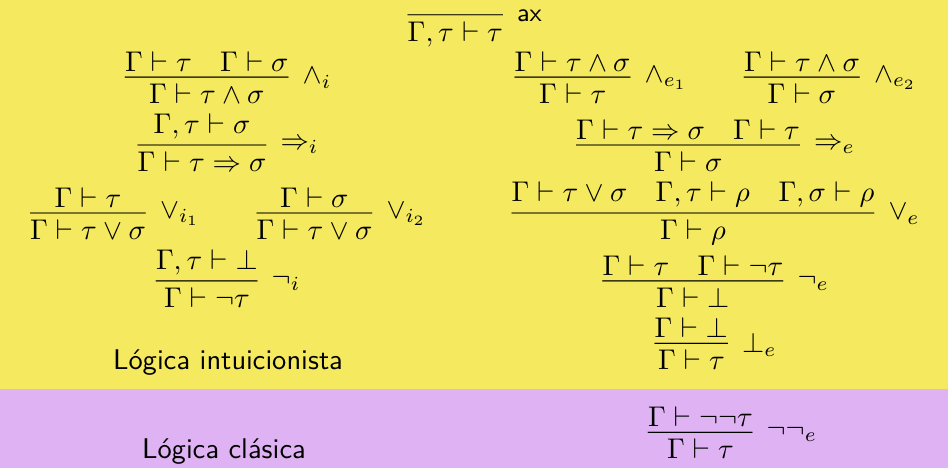
\includegraphics[width=\linewidth]{assets/logica_1.png}
\end{minipage}\]
\[\begin{minipage}[b]{0.5\textwidth}
    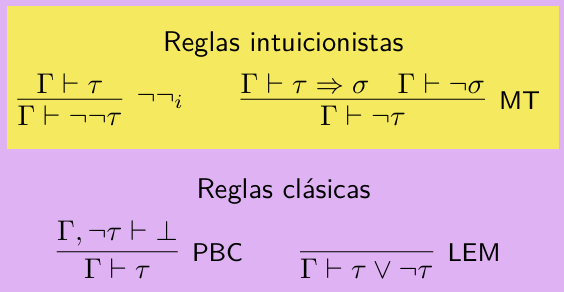
\includegraphics[width=\linewidth]{assets/logica_2.png}
\end{minipage}\]
\subsection*{Weakening (Debilitamiento) y Strengthening (Fortalecimiento)}
\textbf{Weakening}: Lo voy a decir en criollo, su demostración se hace por inducción, pero básicamente es que si algo se cumple solo con \textbf{$\tau$} entonces si agrego otras hipótesis también seguirá valiendo. \\
Se dice que es Weakening porque estamos haciendo más débil la prueba, esto es porque a mayor cantidad de información que tiene el contexto es más dificil de probar. \\
\begin{center}
    \sd{}{\Gamma \vDash \sigma}{} $\implies$ \sd{}{\Gamma, \tau \vDash \sigma}{}
\end{center}
\textbf{Strengthening}: Es lo contrario a Weakening, la idea es que podemos ir sacando hipótesis que no nos sirven y poder seguir probando que vale. Se utiliza mucho en algo llamado Cálculo Lambda que veremos luego. \\
Se dice que es Strengthening porque estamos haciendo más fuerte la prueba, esto es porque a menor cantidad de información que tiene el contexto es más fácil de probar.
\subsection*{Correctitud (Soundness) y Completitud}
\textbf{Importante}: Utilizamos $\vDash$ para hablar de satisfacibilidad en el contexto de \textbf{semántica} mientras que utilizamos $\vdash$ para indicar que una fórmula se puede derivar en el contexto de \textbf{sintáxis}. \\

Correctitud y Completitud responde a la siguiente pregunta: ¿cuál es la relación entre la sintáxis y la semántica?
\begin{itemize}
    \item \textbf{Sintáxis}: Conjunto de fórmulas $\tau$ tal que $\neg \tau$ es un secuente válido. 
    \item \textbf{Semántica}: Conjutno de fórmulas $\tau$ tal que $v \vDash \tau$ para toda valuación $v$. Ej: Tautologías.
\end{itemize}
\[\Gamma \vDash T \iff \Gamma \vdash T\]
\textbf{Corrección} \\
$\vDash \tau$ secuente válido implica que $\tau$ es tautología.
\begin{itemize}
    \item $\sigma_{1}, \sigma_{2}, \dots, \sigma_{n} \vdash \tau$ secuente válido implica que $\sigma_{1}, \sigma_{2}, \dots, \sigma_{n} \vDash \tau$
\end{itemize}
\textbf{Para demostrar}: Hacemos inducción en la estructura de la prueba analizando por casos la última regla aplicada en la prueba. \\
Caso base, la última regla fue un axioma. \\
Casos recursivos, el resto de reglas $\land_{i}, \land_{e1}, etc$ \\
\textbf{Completitud}
$\tau$ tautología implica que $\vdash \tau$ es secuente válido. 
\begin{itemize}
    \item $\sigma_{1}, \sigma_{2}, \dots, \sigma_{n} \vDash \tau$ implica que $\sigma_{1}, \sigma_{2}, \dots, \sigma_{n} \vdash \tau$ es un secuente válido. 
\end{itemize}
\textbf{Para demostrar}: Usamos el contrarrecíproco: si $P \implies Q$ vale que $\neg Q \implies \neg P$ \\
Luego probar estos dos lemas
\begin{itemize}
    \item Si $\Gamma \nvdash \tau$ entonces $\Gamma \cup \{\neg \tau\}$ es consistente (sale por contrarrecíproco).
    \item Si $\Gamma$ es consistente, entonces tiene modelo. Ej.: $\Gamma$ es satisfactible (es más dificil).
\end{itemize}
\subsection*{Consecuencia Semántica}
Sean $\tau_{1}, \tau_{2}, \dots, \tau_{n}, \sigma$ fórmulas de la lógica proposicional. \\
$\tau_{1}, \tau_{2}, \dots, \tau_{n} \vDash \sigma \iff \forall \ v \ valuacion \ ((v \vDash \tau_{1} \land v \vDash \tau_{2} \land \dots \land v \vDash \tau_{n}) \implies (v \vDash \sigma))$ \\
\textbf{En criollo}: Vale que $\tau_{1}, \tau_{2}, \dots, \tau_{n} \vDash \sigma \iff$ para toda valuación v tal que v satisface a todas las hipótesis $v \vDash \tau_{i}$ para toda $i \in 1, \dots, n \implies v \vDash \sigma$ 
\subsection*{Consistencia}
Decimos que $\Gamma$ es consistente si $\Gamma \nvdash \bot$, es decir, $\Gamma$ es consistente si no se puede derivar una contradicción a partir de él.
\section*{Cálculo Lambda ($\lambda$)}
\subsection*{Con booleanos}
Definamos algunas cosas 
\begin{itemize}
    \item \textbf{Tipos}: $\tau, \sigma, \rho, \dots ::= bool \ | \ \tau \rightarrow \sigma$. 
    Asumimos que el constructor de tipos $\leftarrow$ es asociativo a derecha.
    \item \textbf{Términos}: Variables $X = \{X, Y, Z, \dots\}$
    \item \textbf{Construcción explícita de función (sin nombre)}: $\lambda x . M$ 
    \item \textbf{Aplicación de una función a un argumento}: $MN$ 
    \item \textbf{Constantes para cada valor de verdad}: true y false.
\end{itemize}
\textbf{Observación}: Todo es una función, es decir, una función tomando un argumento constante u otra función es lo mismo. \\
Ej.: Una función que toma una función y la compone consigo misma es $\lambda f . \lambda x . f(fx)$ \\
\textbf{Observación 2}: No existen funciones que tomen varios argumentos. \\ 
Ej.: $f(x,y) = $ if $y$ then $x$ else true en cálculo lambda se escribe $\lambda y . \lambda x . if \ x \ then \ y \ else \ true$ \\
\textbf{Observación 3}: La aplicación asocia a la izquierda: $F \ false \ true = (F \ false) true$ \\
\textbf{Observación 4}: La abstracción y el if tienen menor precedencia que la aplicación. \\
Ej.: $\lambda x:\tau . M \ N = \lambda x : \tau . (M \ N) \neq (\lambda x : \tau . M) N$ 
\subsubsection*{Gramática del cálculo lambda con booleanos}
Los términos válidos de cálculo lambda con booleanos los podemos describir con una gramática formal 
\[M \ ::= \ x \ |\  \lambda x \ . \ M \ | \ MM \ | \ true \ | \ false \ | \ if \ M \ then \ M \ else \ M\] 
\subsection{Tipos en Cálculo Lambda}
En el Cálculo Lambda tipado damos los tipos en las operaciones. \\
Ej.: $\backslash \lambda x:\sigma \ . \ M$
\subsection*{Función Identidad}
En cálculo lambda existe una función id \textbf{propia por cada tipo}.
\subsection{Semántica Operacional}
La \textbf{gramática} nos dice qué terminos podemos escribir sintácticamente. \\
La \textbf{semántica} nos da el significado de los términos. \\
Las siguientes reglas tienen la forma $M \rightarrow N$ y se lee $M \ reduce \ a \ N$ o $M \ se \ reescribe \ como \ N$ \\
\begin{itemize}
    \item $(\lambda x . M) N \rightarrow M \{x := N\}$ ($\beta$ reducción)
    \item if true then $M$ else $N \rightarrow M$ ($if_{t}$)
    \item if false then $M$ else $N \rightarrow N$ ($if_{f}$)
\end{itemize}
\subsubsection{Captura de variables}
$\lambda x:bool \ . \ x \equiv $ boolean main(boolean var)$\{return \ x\}$ \\
Cuando las variables están ligadas a un cuantificador podemos cambiarle el nombre sin problema alguno (pensar en el nombre de un parámetro de función en un lenguaje imperativo). \\
Ej.: $x \ (\lambda x:bool \ . \ x) \equiv x \ (\lambda y:bool \ . \ x)$ \\
Esto de que cambiar el nombre de la variable ligada al cuantificador se debe a que son clases de equivalencia ($\alpha$).

\subsubsection{Conjunto de Variables Libres}
Se denota como $fv(M)$.
\subsection{Sistema de Tipos}
Hasta ahora veníamos utilizando tipos estrictos, pero normalmente el Cálculo Lambda \textbf{no viene tipado}. \\
Los tipos de cálculo lambda con booleanos los definimos inductivamente por 
\begin{itemize}
    \item Bool es un tipo.
    \item Si $\tau$ y $\sigma$ son tipos, $\tau \rightarrow \sigma$ es un tipo que representa las funciones de $\tau$ en $\sigma$.
\end{itemize}
Gracias a los tipos, debemos escribir \textbf{de qué tipo son cada una de las variables}. \\
\textbf{Importante}: Solo nos vamos a interesar en \textbf{términos sin variables libres}, es suficiente con escribir el tipo cuando se liga la variable. \\
\textbf{Nota}: Solo los subtérminos tendrán variables libres. \\
Ej.: $\lambda x:Bool . x$ es la identidad sobre los booleanos. \\
Ej.: $\lambda x:Bool \rightarrow Bool.x$ es la identidad sobre las funciones de booleanos en booleanos. \\

La gramática de cálculo lambda con booleanos tipado la definimos con una \textbf{gramática de tipos} y una de \textbf{términos} de la siguiente manera
\begin{itemize}
    \item $\tau :: = Bool \ | \ \tau \rightarrow \tau$
    \begin{itemize}
        \item Nota: $\tau \rightarrow \tau$ representa una función.
    \end{itemize}
    \item $M ::= x \ | \ \lambda x: \tau . M \ | \ M M \ | \ tt \ | \ ff \ | \ if \ M \ then \ M \ else \ M$
\end{itemize}
Donde $M$ representa un término y $\tau$ el tipo. \\
\subsection{Contexto}
Dijimos anteriormente que solo damos tipo a los \textbf{términos sin variables libres} pero ¿que pasa con este caso: $\lambda x:Bool.yx$? \\
Podemos notar que $y$ es una variable libre, y como estamos usando tipos booleanos tiene que ser una función Bool en algo pero ¿como defino ese algo? \\
Un \textbf{contexto} nos da tipos para variables, entonces en vez de decir $\lambda x:Bool.yx:Bool \rightarrow Bool$ decimos, si $y:Bool \rightarrow Bool$, entonces $\lambda x:Bool.yx : Bool \rightarrow Bool$ \\
\textbf{Notación}: $y: Bool \rightarrow Bool \vdash \lambda x: Bool.yx : Bool \rightarrow Bool$ donde del lado izquierdo del $\vdash$ definimos el contexto.
\subsubsection{Contexto de Tipado}
Es un conjunto finito de pares $(x_{i}:\tau_{i})$ 
\[\{x_{1}:\tau_{1}, \dots, x_{n}:\tau_{n}\}\]
\textbf{Nota}: Lo notamos con letras griegas mayúsculas $(\Gamma, \triangle)$ y \textbf{sin variables repetidas}, es decir, $(i \neq j \implies x_{i} \neq x_{j})$
\subsubsection{Juicios de Tipado}
El sistema de tipos predica sobre \textbf{juicios de tipado} de la forma: $\Gamma \vdash M:\tau$ \\
Se lee como ``en el contexto $\Gamma$, $M$ es de tipo $\tau$``
\[\begin{minipage}[b]{1\textwidth}
    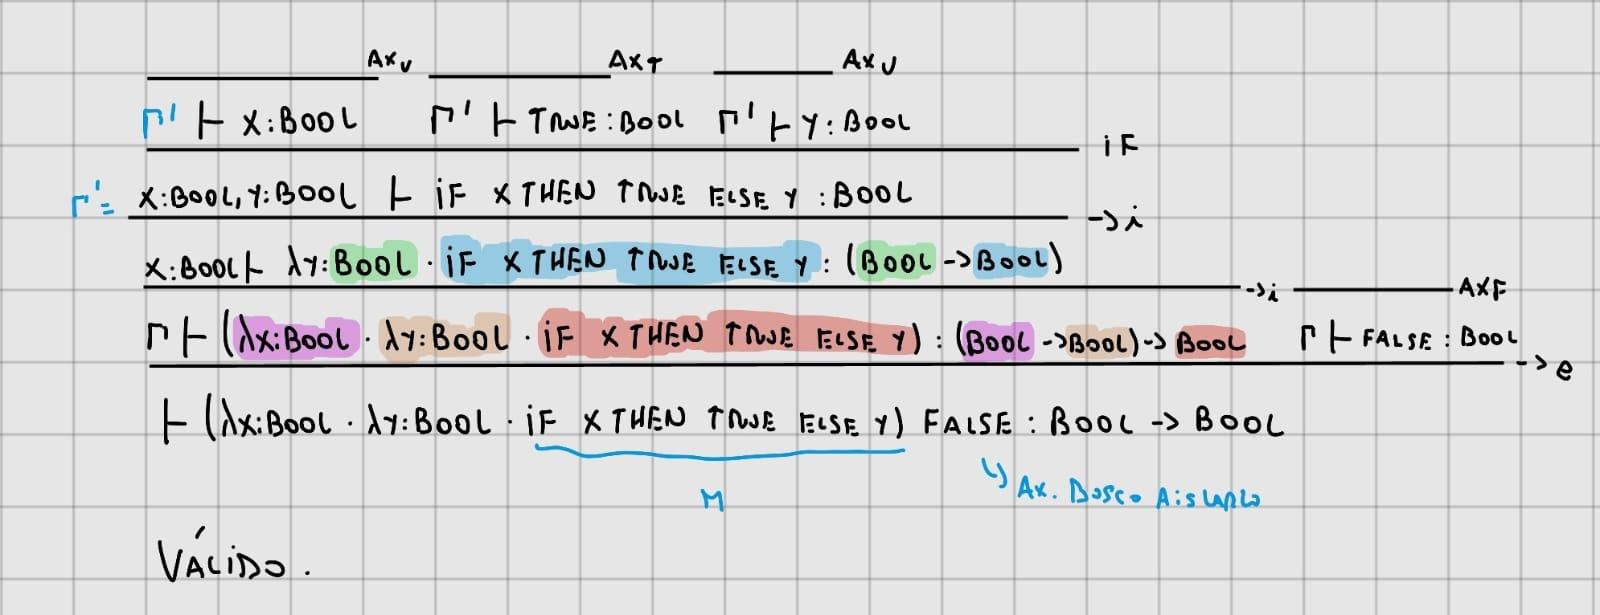
\includegraphics[width=\linewidth]{assets/tipado.jpg}
\end{minipage}\]
\subsection{Sistema de tipos}
La relación de tipado $\Gamma \vdash M:\tau$ se define inductivamente por: 
\[\begin{minipage}[b]{1\textwidth}
    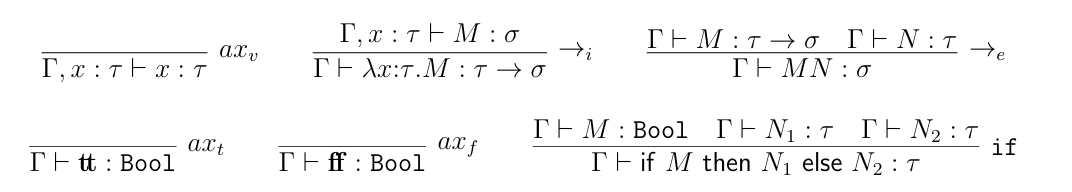
\includegraphics[width=\linewidth]{assets/sistema_tipos.png}
\end{minipage}\]
donde 
\begin{itemize}
    \item $ax_{v}$: variable 
    \item $ax_{t}$: true 
    \item $ax_{f}$: false
    \item $\rightarrow_{i}$: abstracción
    \item $\rightarrow_{e}$: aplicación
    \item $if$: condicional
\end{itemize}
\textbf{Importante}: Es posible que también se utilice la siguiente notación. 
\[\begin{minipage}[b]{0.7\textwidth}
    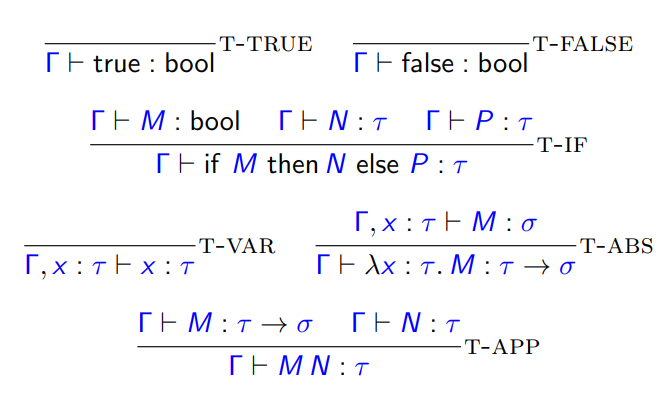
\includegraphics[width=\linewidth]{assets/tipado_operaciones2.png}
\end{minipage}\]
\subsubsection{Árbol Sintático}
Es muy útil hacerlo. \\ 
Véase \hyperref[subsec:arbol_sintatico]{\textbf{\underline{anexo}}} para ver ejemplos para reducir expresiones y verificar si son términos. 
\subsubsection{Término Bueno}
Decimos que un término es bueno si existe un contexto del que puedo derivarlo. 
\subsubsection{Término Válido}
Está atado a como está sintácticamente formado. Es importante que solo tengan tipos válidos.
\begin{itemize}
    \item $x M$: No es válido. No podemos usar genéricos como M.
    \item $\lambda x:Bool$: No es válido. Las funciones toman algo y devuelven algo. Esta lambda no es $\tau \rightarrow \tau$.
    \item $\lambda x.x$: No es válido. No sabemos el tipo de x.
    \item if $x$ then $\lambda x:Bool x$: No es válido, los condicionales tienen una rama else.
    \item $\lambda x: Bool \rightarrow Bool . xy \ \lambda y: Bool . x$
    \begin{itemize}
        \item Si colocamos los paréntesis de la asociación queda así: $((\lambda x: Bool \rightarrow Bool . x \textbf{y}) \ (\lambda y: Bool . \textbf{x}))$
        \item Por un lado se resuelve $(\lambda x: Bool \rightarrow Bool . xy)$ y por otro $(\lambda y: Bool . x)$.
        \item Finalmente, cuando reduce, se realiza la aplicación. En negrita, están marcadas las variables libres.
        \item Este término es válido.
    \end{itemize}
    \item $\lambda y:\sigma . y$: No es válido, no existe el tipo $\sigma$. Solo existe $Bool \ | \ \tau \implies \tau$
    \item $xy \ \lambda x: Bool \rightarrow Bool . xy$
    \begin{itemize}
        \item Asociemos hacia la izquierda entonces queda $(xy) \ (\lambda x: Bool \rightarrow Bool . xy)$
        \item Cada lado se resuelve por separado y luego se componen.
    \end{itemize}
\end{itemize}
Para ver ejemplos de esto utilizando árboles sintáticos véase \hyperref[subsec:arbol_sintatico]{\textbf{\underline{anexo}}}
\subsubsection{Término Cerrado}
Decimos que un término es cerrado sí y solo sí no tiene variables libres.
\subsubsection{Contexto Vacio}
Un contexto está vacío si no existe ninguna variable libre.
\subsubsection{Tipando operaciones}
\[\begin{minipage}[b]{0.8\textwidth}
    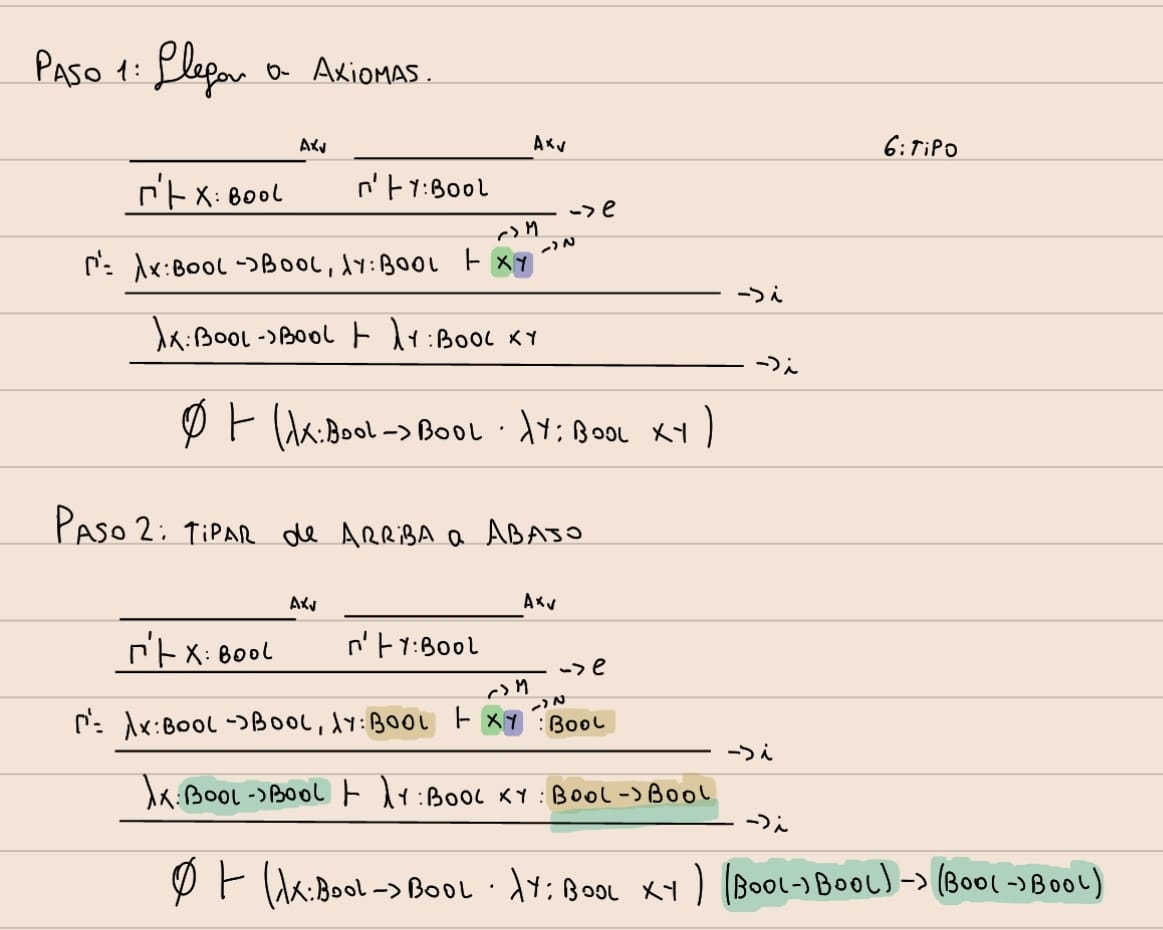
\includegraphics[width=\linewidth]{assets/tipado_operaciones.jpg}
\end{minipage}\]
\[\begin{minipage}[b]{0.8\textwidth}
    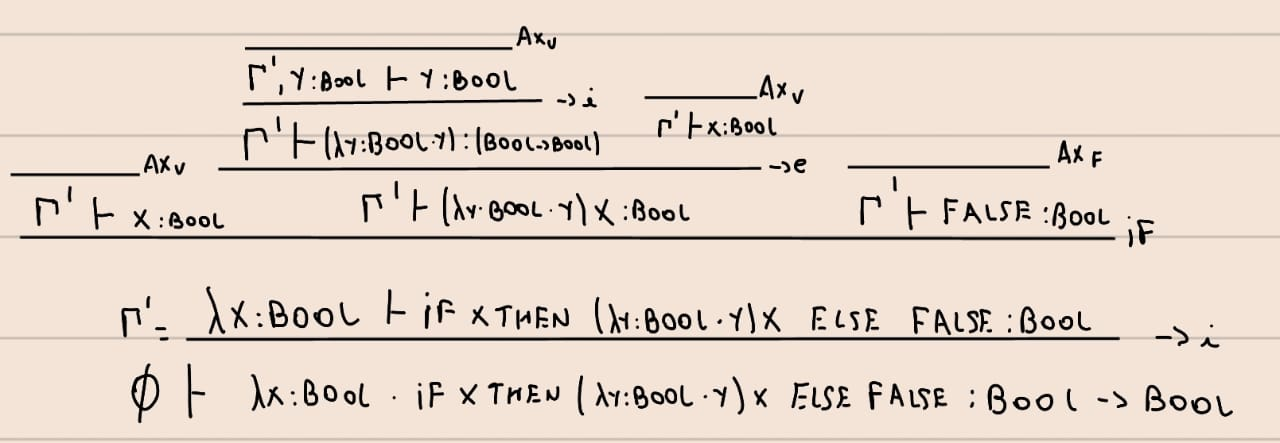
\includegraphics[width=\linewidth]{assets/tipado_condicional.jpg}
\end{minipage}\]
\subsubsection{Clases de Equivalencia (Alfa equivalencia)}
Los términos que difieren sólo en el nombre de las variables $ligadas$ se consideran iguales: $\lambda x:bool \ . \ x \equivDef{\alpha} \lambda y:bool \ xy$
\subsubsection{Aplicando Clases de Equivalencia}
Recordemos que las variables ligadas, en cualquier lenguaje de programación serían como el parámetro de una función y da igual que nombre le pongamos. Lo importante es NO tener dos parámetros con el mismo nombre.
\[\begin{minipage}[b]{0.9\textwidth}
    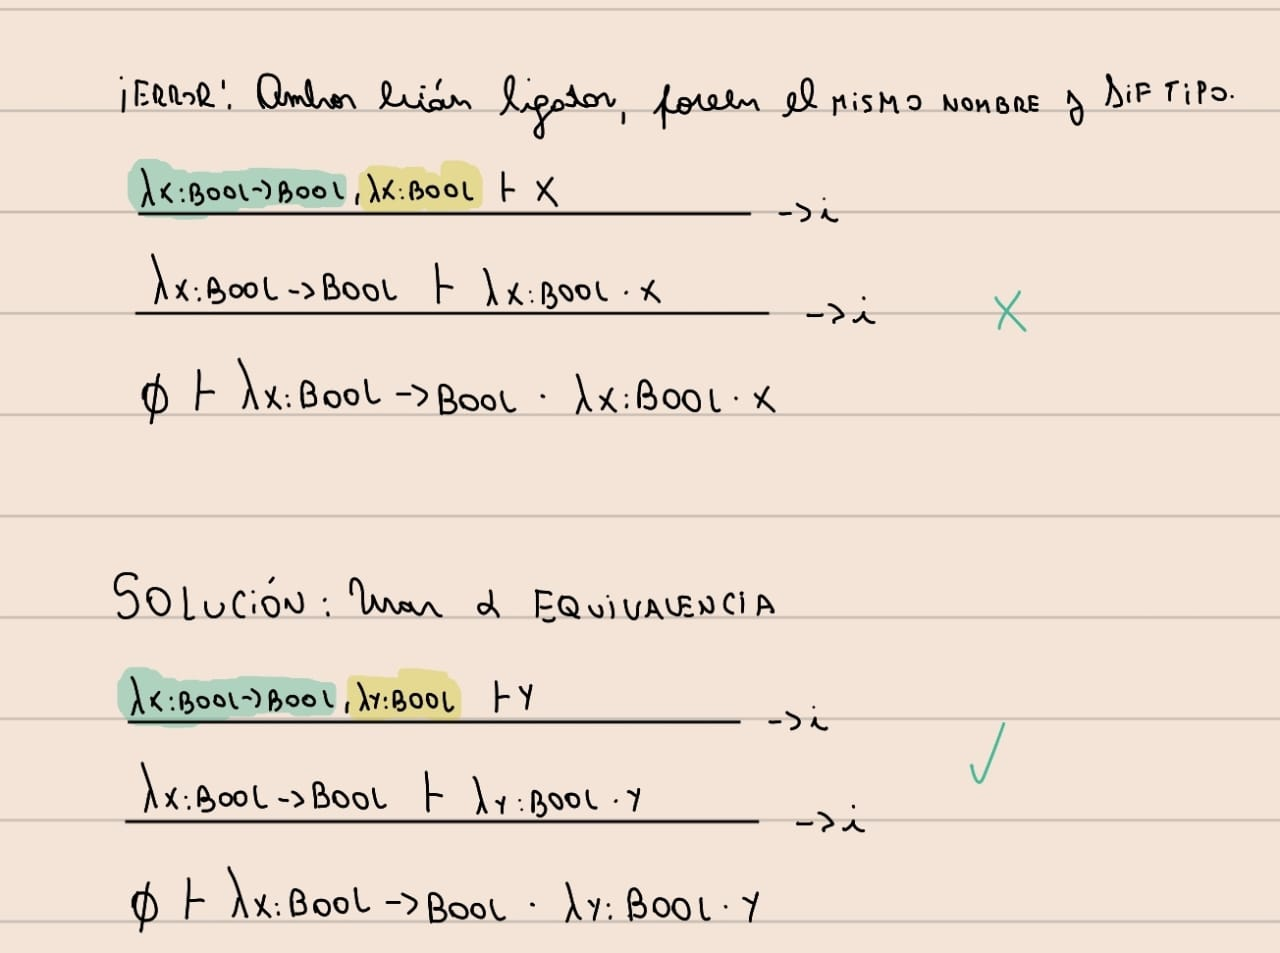
\includegraphics[width=\linewidth]{assets/alfa_reduccion.jpg}
\end{minipage}\]
\textbf{Nota}: Al igual que en un lenguaje de programación da igual a qué variable ligada le cambiemos su nombre.
\subsubsection{Unicidad de Tipos}
Si $\Gamma \vdash M:\sigma$ y $\Gamma \vdash M:\rho$ ent $\sigma = \rho$ 
\subsubsection{Teorema (Weakening + Strengthening)}
Si $\Gamma \vdash M:\tau$ es derivable y $fv(M) \subseteq \Gamma \cap \Gamma'$ entonces $\Gamma' \vdash M:\tau$ es derivable
\begin{itemize}
    \item Weakening: Agregar más hipótesis hace que la afirmación sea más débil y dificil de demostrar.
    \item Strengthening: Sacar hipótesis hace que la afirmación sea más fuerte y fácil de demostrar.
\end{itemize}
Veamos un ejemplo de Strengthening: $x:Bool \vdash True:Bool$ \\
Hagámosnos una pregunta ¿utilizamos en algún lado la x? No, entonces tenemos que preguntarnos ¿realmente la necesitamos en el contexto? No. Entonces podemos quitarla y la afirmación será aún más fuerte. \\
Entonces $\emptyset \vdash True:Bool$
\subsection{Tipos Habitados}
Un tipo está habitado si existe una función de ejemplo que use ese tipo. \\
Por ejemplo, si nos piden algo que cumpla $\vdash M:(\tau \rightarrow \rho) \rightarrow (\sigma \rightarrow \tau) \rightarrow (\sigma \rightarrow \rho)$. \\
Podemos notar que una función que haga esto, sería la composición: $\lambda f:\tau \rightarrow e . \lambda g :\sigma \rightarrow \tau . \lambda x:\sigma . f (gx)$ o mejor escrita $(\lambda f:\tau \rightarrow e) (\lambda g :\sigma \rightarrow \tau)(\lambda x:\sigma) (f (gx))$
\subsection{Semántica Formal}
El sistema de tipos nos indica cómo se construyen los programos pero además queremos darles \textbf{significado} (semántica).
Existen tres formas de dar semántica formal 
\begin{itemize}
    \item \textbf{Semántica Operacional}: Indica cómo se ejecuta el programa hasta llegar a un resultado.
    \begin{itemize}
        \item Es la que vamos a usar en la materia.
        \item Trabaja en base a reglas de reducción $\rightarrow$ entre términos. Cuando tenemos $M\rightarrow N$, M reduce. 
        \item La idea es llegar a formas normales, es decir, expresiones irreducibles que no existe ninguna regla que las pueda deducir.
        \item small-step: ejecución paso a paso.
        \item big-step: evaluación directa al resultado.
    \end{itemize}
    \item \textbf{Semántica Denotacional}:  Interpreta los programas como objetos matemáticos.
    \item \textbf{Semántica Axiomática}: Establece relaciones lógicas entre el estado del programa antes y después de la ejecución.
\end{itemize}
\textbf{Importante}: Nosotros vamos a usar la estrategia de reducción call by value, y nos va a interesar mantener el determinismo de las reglas de reducción.
\subsection{Semántica Operacional}
\subsubsection{Small-Step}
La semántica operacional predica sobre \textbf{juicios de evaluación}: $M \rightarrow N$ donde M y N son programas. 
\subsubsection{Valores}
Los valores son los posibles resultados de evaluar programas: $V::=true \ |\ false \ | \ \lambda x: \tau.M$ 
\subsection{Semántica Operacional}
\[\begin{minipage}[b]{0.9\textwidth}
    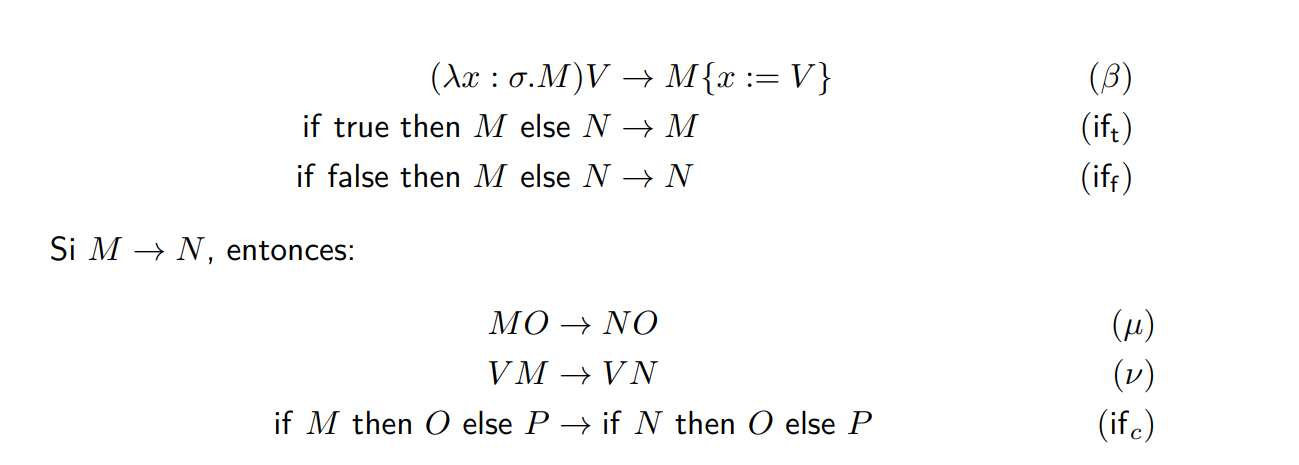
\includegraphics[width=\linewidth]{assets/reglas_congruencia_computo.png}
\end{minipage}\]
\textbf{Importante}: $\mu$, $v$, $if_{c}$ son reglas de congruencia, es decir, nos permiten ``ingresar a la expresión para luego aplicar las reglas de cómputo`` las cuales, las reglas de compúto son $\beta, (if_{t}), (if_{f})$ \\
\textbf{Importante 2}: Aplicar la regla $\beta$ NO cuenta como regla de redudcción. \\
\textbf{Importante 3}: $\beta$ se utiliza \textbf{SOLO} con valores. \\
\textbf{Importante 4}: Recordar que $\rightarrow$ indica a qué reduce, por ejemplo, en el caso del if false, tiene sentido que si el else es N, la operación te devuelva N. \\
Veamos a continuación unos ejemplos 
\[\begin{minipage}[b]{0.9\textwidth}
    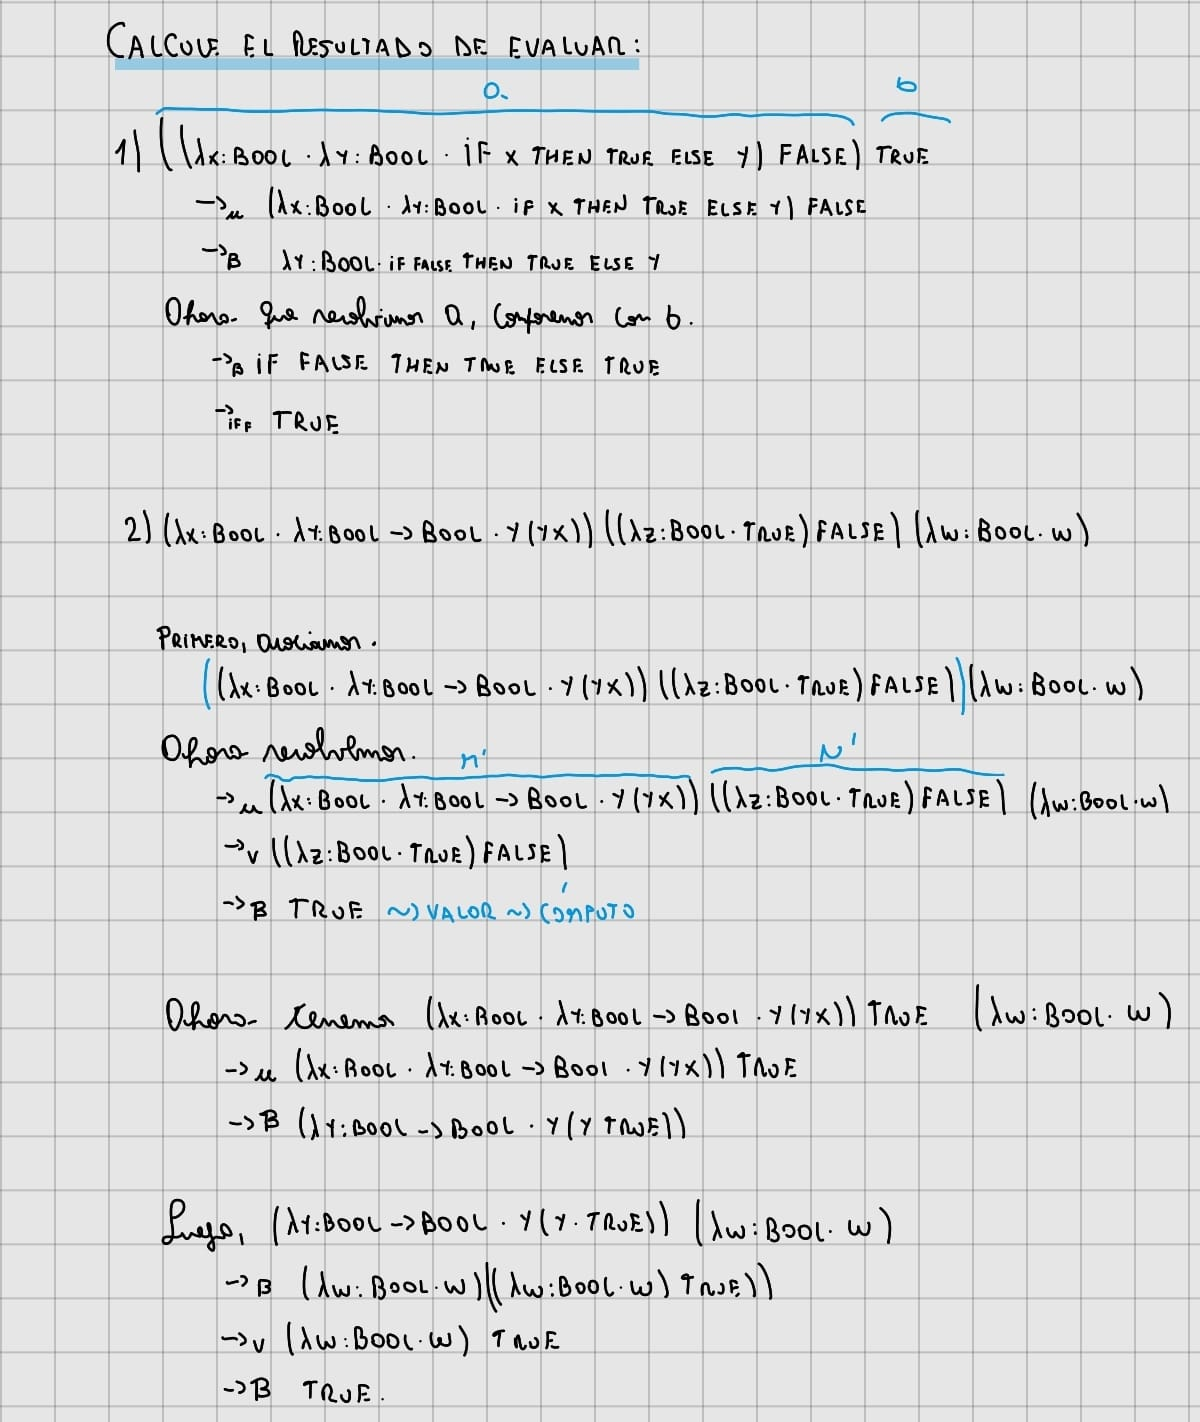
\includegraphics[width=\linewidth]{assets/semantica-operacional-ej.jpg}
\end{minipage}\]
\subsubsection{Sustitución}
La operación de sustitución $M\{x:=N\}$ nos devuelve un nuevo término tal que resulta de reemplazar todas las ocurrencias libres de x en M por N. \\
\textbf{Nota}: Se implementa por pattern matching porque es un constructor recursivo. 
\[\begin{minipage}[b]{0.8\textwidth}
    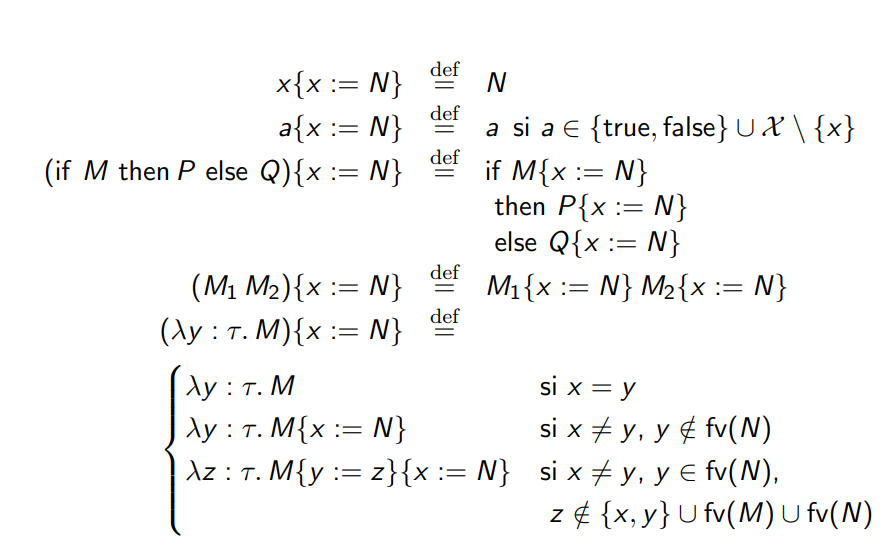
\includegraphics[width=\linewidth]{assets/def_sustitucion.png}
\end{minipage}\]
\subsection{Propiedades de la Evaluación}
\subsubsection{Teorema (Determinismo)}
Si $M \rightarrow N_{1}$ y $M \rightarrow N_{2}$ entonces $N_{1} = N_{2}$ \\
\textbf{En criollo}: No hay más de una forma de reducir algo. 
\subsubsection{Teorema (Preservación de Tipos o Subject Reduction)}
Si $\Gamma \vdash M : \tau$ y $M \rightarrow N$ entonces $\Gamma \vdash N:\tau$ \\
Si deducimos el tipo $\tau$ para un término sin ejecutar el programa, y luego ejecutamos el programa obteniendo N, entonces el término N tiene el mismo tipo. 
\subsubsection{Teorema (Progreso)}
Si $\vdash M:\tau$ entonces: 
\begin{itemize}
    \item O bien M es un término cerrado irreducible bien tipado, osea un valor. 
    \item O bien existe un $N$ tal que $M \rightarrow N$
\end{itemize}
\subsubsection{Teorema (Terminación)}
Si $\vdash M:\tau$ entonces no hay una cadena infinita de pasos: $M \rightarrow M_{1} \rightarrow M_{2} \rightarrow ...$
\subsubsection{Canonicidad}
\begin{itemize}
    \item Si $\vdash M:bool$ es derivable, entonces la evaluación de M termina y el resultado es true o false.
    \item Si $\vdash M:\tau \rightarrow \sigma$ es derivable, entonces la evaluación de M termina y el resultado es una abstracción. 
\end{itemize}
\subsubsection{Extensión con Números Naturales}
Sintaxis:
\[\begin{minipage}[b]{0.8\textwidth}
    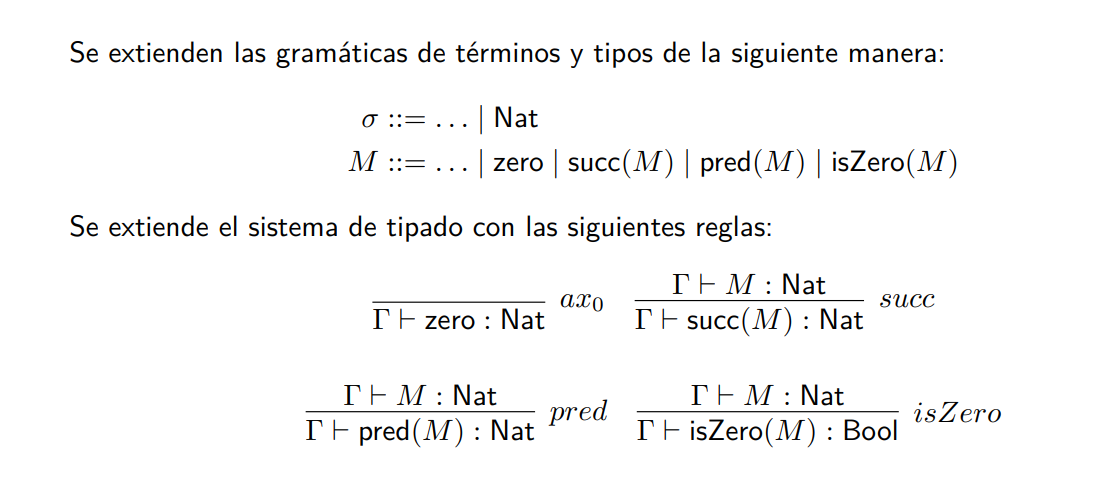
\includegraphics[width=\linewidth]{assets/extension_naturales.png}
\end{minipage}\]
Semántica:
\[\begin{minipage}[b]{0.8\textwidth}
    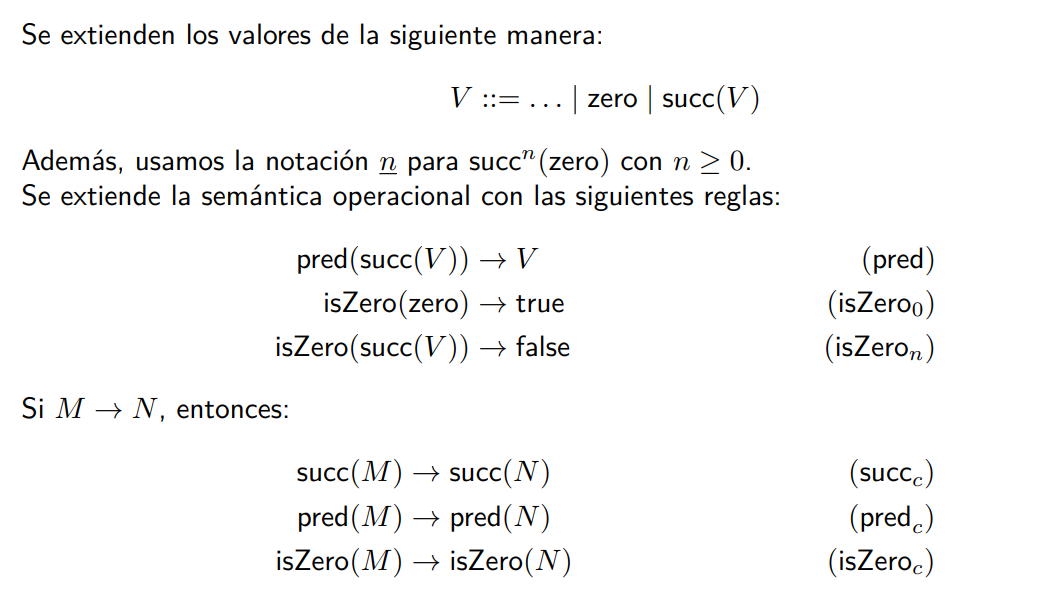
\includegraphics[width=\linewidth]{assets/extension_naturales_semantica.png}
\end{minipage}\]
\textbf{Ultra Importante}: Cada vez que extendmos tipos o sintaxis hay que chequear que siga valiendo el progreso, el determinismo y la preservación de tipos. \\
\textbf{¿Es segura esta extensión?}: No, porque con estas reglas se rompe el progreso pues pred(0) es forma normal pero no es un valor válido. \\
Si quisieramos que siga valiendo el progreso podemos extender la semántica y agregar un caso \textbf{$pred(zero) \rightarrow zero$ ($pred_{0}$)}
\subsubsection{Macros}
\[\begin{minipage}[b]{0.8\textwidth}
    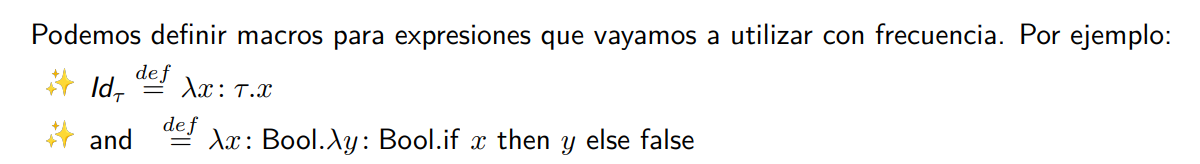
\includegraphics[width=\linewidth]{assets/macros.png}
\end{minipage}\]
\subsubsection{Agregando Reglas para las Abstracciones}
\[\begin{minipage}[b]{0.8\textwidth}
    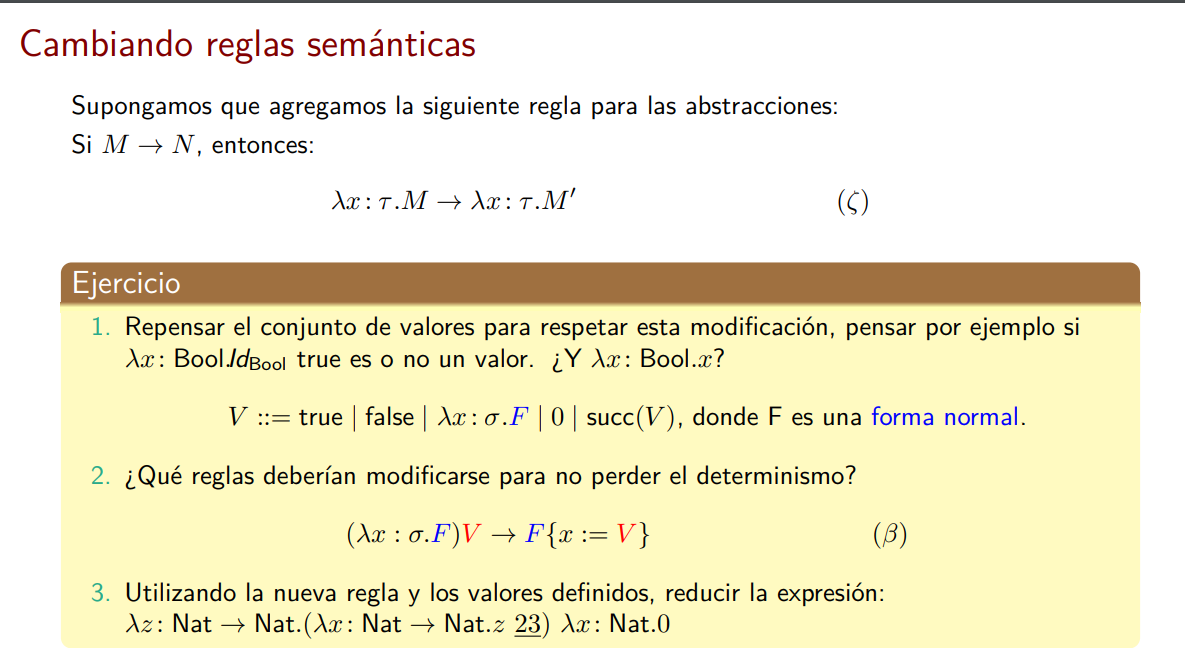
\includegraphics[width=\linewidth]{assets/forma_normal.png}
\end{minipage}\]
(No entendí qué caso es el conflictivo si tuvimos que cambiar de $\lambda x: \sigma . M$ a $\lambda x:\sigma . F$) ¿qué no podíamos hacer antes?
\section*{Anexo}
\subsection*{Recordando Haskell}
Para ejecutar un archivo hay que instalar GHCI. Una vez instalado, nos paramos en la terminal en el directorio donde está el archivo que queremos ejecutar. 
\begin{itemize}
    \item Cargar archivo: :l nombreArchivo
    \item Ver tipo: :type tipo 
    \item Ejecutar funcion: funcion parametro1 parametro2...
    \item Recargar archivo: :r
    \item Si necesitamos hacer cálculos para mandar un parámetro, usar paréntesis: Ej.: otherwise = n * factorial(n-1)
\end{itemize} 
\subsection*{Maybe}
El Maybe se utiliza en Haskell para recibir/devolver respuestas condicionales que pueden ser de un tipo u otro. \\

Se define como $data \ Maybe \ a \ = \ Nothing \ | \ Just \ a$ \\

Ej.: $ devolverFalsoSiVerdadero \:: \ Bool \rightarrow Prelude.Maybe \ Bool $ \\

El Maybe deja la puerta abierta a un valor posible "Nothing". Entonces tenemos dos casos: Si me envian un True devuelvo False (tipo bool), caso contrario, devuelvo Nothing. 

\subsection*{Either}
El Either se utiliza en Haskell para poder recibir/devolver un parámetro que podría ser de un tipo u otro. \\
Se define como $ data \ Either \ a \ b \ = \ Left \ a \ | \ Right \ b $ \\

Para poder saber qué operación hacer según el tipo literalmente en código usamos (Left valor) o (Right valor). \\

Ej.: $ devolverRepresentacionIntBool \ :: \ Either \ Int \ Bool \ \rightarrow \ Int $ \\

Si es un entero, devuelvo ese mismo entero porque no hago nada. Eso lo hacemos con $Left(a) \ = \ a$, ahora, si el tipo es booleano tengo que decir explícitamente la respuesta según su valor. Es decir, $Right(False) \ = \ 0$ sino, $Right(True) \ = \ 1$.

\subsection*{Declaración de tipos en Haskell}
Se utiliza $data \ nombretipo \ tipo \ = \ Tipo \ 1 \ | \ Tipo \ 2$ 
El $|$ se interpreta como \textbf{o bien}
\subsection*{Árboles Binarios}
Es un tipo (para mi parecer) meramente recursivo. \\
$data \ AB \ a \ = \ Nil \ | \ Bin \ (AB \ a) \ a \ (AB \ a)$
Nótese que es algo re contra recursivo, porque para definir el tipo de AB a decimos que es un Bin que a su vez es de AB a y a su vez AB a es otro árbol binario. \
Veamos unos ejemplos de esto
\begin{itemize}
    \item Bin (Nil) Nil (Nil): es el árbol que no tiene ni siquiera raíz. Y nótese que en cada paréntesis es importante indicar el Nil pues es la forma de que el tipado de Haskell nos lo acepte.
    \item Bin (Bin Nil 3 Nil) 4 (Bin Nil 6 Nil): Es el árbol que comienza con un Nodo raíz que tiene el valor de 4. El hijo izquierdo del Nodo con valor 4 es otro árbol binario que tiene como valor 3 en su nodo y no tiene hijos. El hijo derecho del Nodo con valor 4 es otro árbol binario que tiene como valor 6 en su Nodo y no tiene hijos. 
\end{itemize}
Y así sucesivamente, veamos un dibujo para tener algo más visual. \\
El siguiente árbol binario: Bin (Bin (Bin Nil 2 Nil) 3 Nil) 4 (Bin (Bin Nil 5 Nil) 6 Nil) representa el siguiente:
\[\begin{minipage}[b]{0.5\textwidth}
    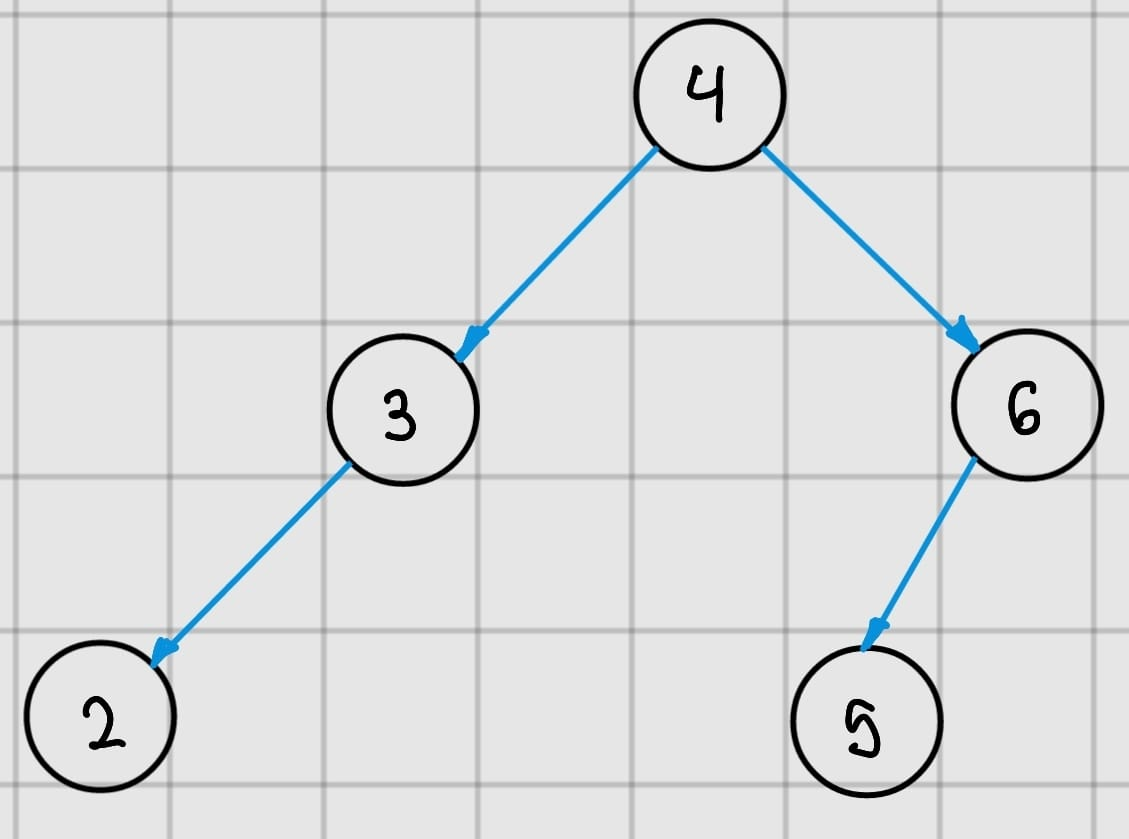
\includegraphics[width=\linewidth]{assets/abb_haskell.jpg}
\end{minipage}\]
\subsection*{Curry \& Uncurry}
\label{subsec:curry_uncurry}
Digamos que necesitamos currificar una función que recibe una tupla de elementos. Es decir, algo así: $ suma :: (Int, Int) -> Int $ \\
Por la definición de curry necesitamos que por cada argumento, haya una función que lo devuelva, por lo tanto el resultado sería algo así $ suma :: Int -> Int -> Int $. \\
Veamos el tipo de función que queremos currificar: $((a, b) -> c)$, esto lo queremos llevar a $a -> b -> c$. \\
Por lo tanto nuestra función curry sería algo así: 
\begin{lstlisting}
    curryOwn :: ((a, b) -> c) -> a -> b -> c
    curryOwn f a b = f (a, b) 
\end{lstlisting}
Entonces, digamos que queremos hacer la suma currificada. 
\begin{lstlisting}
    sumTuple :: (Float, Float) -> Float
    sumTuple (x, y) = x + y

    sumarCurry :: Float -> Float -> Float
    sumarCurry = curryOwn sumTuple
\end{lstlisting}

Lo que hace sumarCurry es llamar a curry(sumTuple) es decir, a curry le manda la función sumTuple. Los parámetros que le mandamos a sumarCurry como a -> b, los convierte en (a, b) para poder aceptar el tipo de la función sumTuple. \\

¿Cómo sería entonces la función uncurry? 
Si recibimos los argumentos en forma de $ a -> b -> c$ debo llevarlo a $ (a, b) -> c$
\begin{lstlisting}
    uncurryOwn :: a -> b -> c -> ((a, b) -> c)
    uncurryOwn f (a, b) = f a b

    sumarUncurry :: (a, b) -> c
    sumarUncurry = uncurryOwn sumarCurry
\end{lstlisting}
Esto quiere decir que vamos a llamar a sumarUncurry que recibe la tupla, ahora sumarCurry está currificada, por lo que la tenemos que convertir nuevamente a la función no currificada, para luego llamar a sumTuple de la manera original.
\subsection*{Clases de Tipos}
\label{subsec:clases_tipos}
\begin{itemize}
    \item Num a: Indica que el parámetro a es numérico
    \item Ord a: Indica que el parámetro a es ordenable bajo algun criterio, es decir, podemos aplicar $ > \ < \ =$ etc.
    \item Eq a: Indica que el parámetro a se puede igualar, es decir, podemos aplicar $=$
\end{itemize}
\subsection*{Foldr}
\label{subsec:foldr_ex}
\begin{lstlisting}
    // Solo recorre listas de tipo a. Es decir, devuelve la suma de los elementos.
    sumFoldrlist :: Num a => [a] -> a 
    sumFoldrlist = foldr (\x ac -> x + ac) 0

    //Recorre tipos plegables. Acá no nos limitamos solo a listas, porque véase que usamos t a en vez de [a]
    sumFoldr :: (Foldable t, Num a) => t a -> a 
    sumFoldr = foldr (\x ac -> x + ac) 0
\end{lstlisting}
\subsection*{Foldr, el árbol de recursión y más de una lista}
\label{subsec:foldr_armar_pares}
Uno de los problemas más normales es tener que enviar más de una lista a procesar a una función dada en Haskell y realizar recursión estructural. \\
Veamos el siguiente ejercicio: Arme pares de la forma [(a, b)] usando recursión estructural. \\
Esto es súper simple si lo hacemos sin recursión estructural porque nos queda algo así 
\begin{lstlisting}
    armarPares :: [a] -> [b] -> [(a, b)]
    armarPares [] _ = []
    armarPares _ [] = []
    armarPares (x:xs) (y:ys) = (x, y) : armarPares xs ys
\end{lstlisting}
¿Cómo hacemos esto con foldr? Veamos el árbol recursivo.
\[\begin{minipage}[b]{0.9\textwidth}
    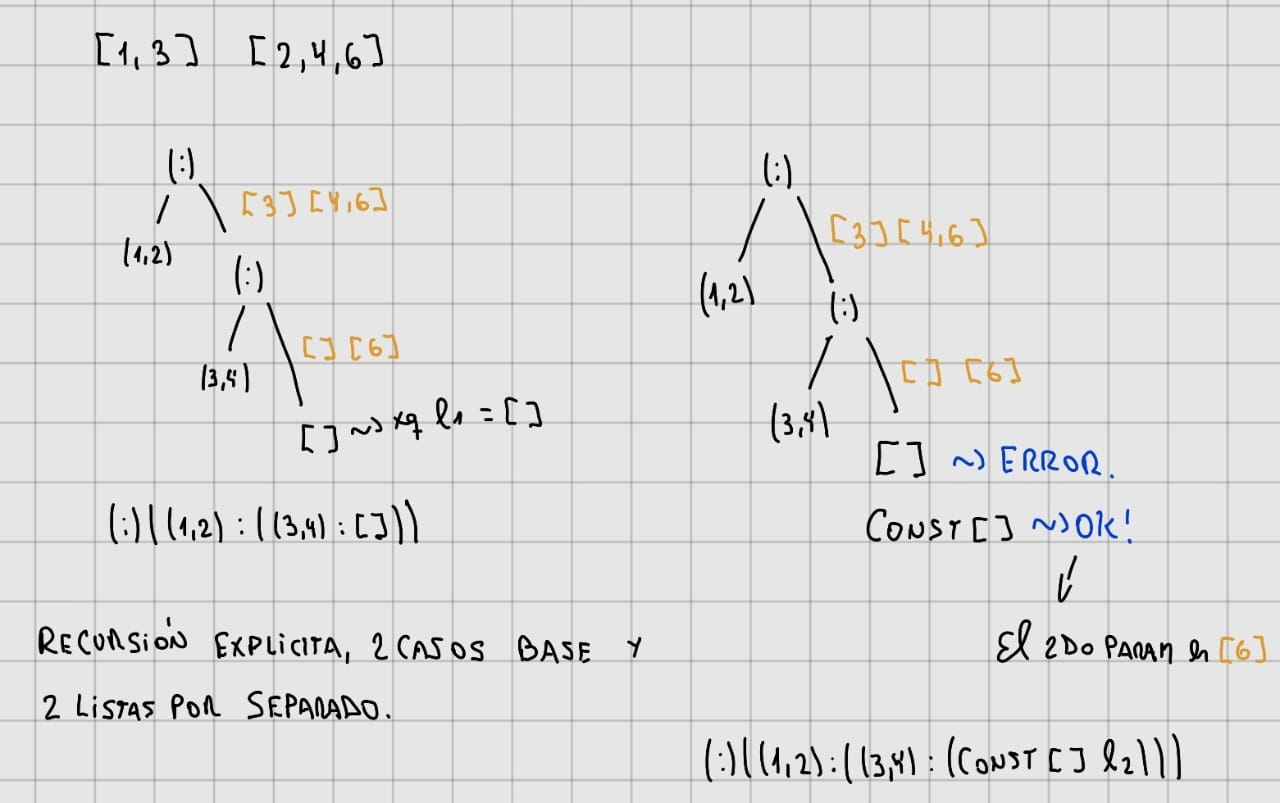
\includegraphics[width=\linewidth]{assets/armar_pares_2.jpg}
\end{minipage}\] 
El error en la recursión estructural vendría del lado de que como estamos recorriendo dos listas a la vez, y mi llamado recursivo es del tipo $[b] \rightarrow [(a,b)]$ no puedo devolver $[]$ entonces lo que hago es devolver $const \ []$ y se aplica parcialmente al argumento que sería la segunda lista $const \ [] \ l2$ y como la primera lista está vacía entonces devuelve []. \\
Esto es súper importante a tener en cuenta, porque si mandamos más de un argumento en la recursión, recordar el concepto de curry.
\subsection*{Flip}
Toma dos parámetros y devuelve una función que los devuelve en el orden inverso. \\
Es decir: $(a \rightarrow b \rightarrow c) \ \rightarrow b \rightarrow a \rightarrow c$ \\
Luego: $ flip \ f \ a \ b \ = \ f \ b \ a $
\subsection*{Función identidad}
Devuelve el mismo valor aplicado a la función. \\
Es decir: $(a  \rightarrow b)  \rightarrow a \rightarrow b$ \\
Luego: $ \$ f \ a \ = \ f \ a  $
\subsection*{Función constante}
Devuelve un valor enviado sin aplicarle ninguna función. \\
Es decir: $a \rightarrow b \rightarrow a$ \\
Luego: $const \ a \ b \ = \ a$
\subsection*{Reduciendo expresiones elegantemente}
\begin{itemize}
    \item $filter(\backslash x \rightarrow length \ x > 3)$
    \begin{itemize}
        \item  ¿Puede hacerse algo mejor? No. Porque a x si o sí necesitamos aplicarle una función.
    \end{itemize}
    \item $filter(\backslash x \rightarrow x > n)$
    \begin{itemize}
        \item ¿Puede hacerse algo mejor? Sí. $filter (>n)$
    \end{itemize}
    \item $filter (\backslash x \rightarrow mod x 2 /= 0)$
    \begin{itemize}
        \item ¿Puede hacerse algo mejor? No. Porque a x le tenemos que calcular su módulo con 2.
    \end{itemize}
    \item $map(\backslash x \rightarrow map (\backslash y \rightarrow toUpper \ y) \ x)$
    \begin{itemize}
        \item ¿Puede hacerse algo mejor? Primero entendamos que hace, recorre una lista de palabras, luego en cada palabra toma cada letra y la pasa a mayúscula. Esto es un doble map, uno por palabra otro por letra. Entonces sí $map \ (map \ toUpper)$
    \end{itemize}
    \item $doblarElementos . filtrarPares$
    \begin{itemize}
        \item ¿Puede hacerse algo mejor? No. Esto es el equivalente a un lenguaje imperativo hacer doblarElementos(filtrarPares(lista))
    \end{itemize}

\end{itemize}
\subsection*{¿Qué hacen las siguientes funciones compuestas?}
\begin{lstlisting}
    flip($) 0 id 

    (==0) . (flip mod 2)

    Primero veamos que hace flip mod 2.
    mod 2 es notación infija (Integral a => 2 -> a -> a), entonces lo que está diciendo es que si le paso cualquier número va a hacer mod 2 x, y nosotros por lo que yo entiendo es que queremos ver si es par.
    Por lo tanto, lo primero que haríamos es invertir los argumentos de mod 2 con flip (Integral a => a -> 2 -> a), entonces quedaría algo como mod x 2 donde el x lo tenemos que enviar nosotros.
    Luego, se compone la función de mod x 2 == 0 esperando solo un argumento donde verifica si efectivamente un número dado es par. 
    Entonces, (Integral a => x -> Bool)
    
    map f = ((:) . f)
    Lo que hace esta función es básicamente aplicar una función f a todos los elementos y agregarlos a una lista particular.
    
    Dado ["hola", "abc"] quiero devolver ["cba", "aloh"]. Es decir, dar vuelta cada caracter de cada palabra y ademas dar vuelta las palabras. 

    reverseAnidado :: ["String"] -> ["String"]
    reverseAnidado = reverse . (map . reverse) 
    Lo primero que hacemos es hacer un map haciendo reverse por cada caracter de la lista. Luego, reordenamos las palabras en sí.
    El tipo de reverse es: [a] -> [a] pero con los elementos al revés. Entonces, por cada palabra (map) hacemos un reverse y las guardamos.
    Finalmente, nos queda algo así ["aloh", "cba"], nos queda dar vuelta eso, entonces hacemos nuevamente un reverse de toda la lista. ["cba", "aloh"].
    
    listacomp f xs p = [f x | x <- xs, p x]
    listacomp f xs p = map f (filter p xs)
\end{lstlisting}

\subsection*{Ejercicios Foldl}
\label{subsec:foldl_ejercicios}
1. Definir la función sumasParciales que dada una lista de números devuelve otra de la misma longitud que tiene en cada posicion la suma parcial de los elementos de la lista original desde la cabeza hasta la posición actual. \\
Entendamos el enunciado: 
\begin{itemize}
    \item Vamos a usar foldl para ir sumando de izquierda a derecha.
    \item El tipado de foldl es b $\rightarrow$ a $\rightarrow$ b donde b es nuestro primer argumento acumulador y a el elemento.
    \item Necesito de alguna manera tener el valor inmediato anterior. Podemos hacer algo como empezar enviando una lista vacia como caso base, y a medida que vamos haciendo la recursion tomar la cabeza de la lista.
    \item Si la lista esta vacia entonces solo agrego x a la lista de la recursion (primer elemento), si no esta vacia sumo con el elemento de la lista (cabeza) 
    \item Porque foldl labura asi $\rightarrow$ [1, 2, 3]
    \begin{itemize}
        \item 1:[] = [1]
        \item 2 + (head [1]) : [1] = [3, 1]
        \item 3 + (head [3, 1]) : [3, 1] = [6, 3, 1]
        \item Ahora podemos usar reverse y el resultado es [1, 3, 6]
    \end{itemize}
\end{itemize}
Entonces la solución sería algo así: 
\begin{lstlisting}
    sumasParciales :: Num a => [a] -> [a]
    sumasParciales = reverse . foldl(\acc x -> if(length acc > 0) then x+(head acc):acc else x:acc) []
\end{lstlisting}
\subsection*{Ejercicios Map}
\label{subsec:map_ejercicios}
1. Realice una función mapDoble que toma una función currificada de dos argumentos y dos listas de igual longitud y devuelve una lista de aplicaciones de la función a cada elemento correspondiente de las dos listas. \\
Básicamente $f=x+y \ l1 = [1, 2] \ l2 = [3, 4] $ da como resultado $[4, 6]$ \\
Desglosemos el ejercicio en partes 
\begin{itemize}
    \item 1. Lo primero que necesito hacer básicamente es recorrer ambas listas de alguna manera a la vez, y obtener algo como [(1, 3), (2, 4)] y luego aplicar a esa lista de pares la función f.
    Si nos ponemos a pensar, basta con hacer una función que reciba dos listas de tipo [a] y [b] y devuelva una lista de [(a, b)]. 
    \item 2. Una vez que tenemos esta lista de pares, sabemos que la función que nos va a enviar tiene que utilizar ambos elementos a la vez, pero la función es de la forma $a \rightarrow b \rightarrow c$ y esto quiere decir que está currificada pero nuestra lista de pares es de tipo $[(a, b)]$ por lo tanto antes de aplicar f debemos aplicar $ uncurry \ f \ lista$ para que cuando mandemos f y la lista, f se convierta en una función que espere $(a, b)$.
    \item 3. Por último, para aplicar a todos los elementos de la lista podemos usar map de la siguiente forma: $map \ (uncurry f) (lista)$
\end{itemize}
\begin{lstlisting}
    mapDobleCorta :: (a -> b -> c) -> [a] -> [b] -> [c]
    mapDobleCorta f l r = map (uncurry f) (armarPares l r)
\end{lstlisting}
donde la función armarPares tiene la siguiente pinta 
\begin{lstlisting}
    armarPares :: [a] -> [b] -> [(a, b)]
    armarPares _ [] = []
    armarPares [] _ = []
    armarPares (x:xs) (y:ys) = (x, y) : armarPares xs ys 
\end{lstlisting}
2. Realice una suma de matrices.
\begin{itemize}
    \item Idea: Necesitamos de alguna manera recorrer la fila 1 de la matriz 1 y la fila 1 de la matriz 2. Esto lo podemos hacer facilmente reutilizando el ejercicio anterior (armarPares), es decir, enviamos armarPares con la fila1 matriz1 y fila1 matriz2. Esto nos armaría los pares de esa fila. 
    \item Tenemos que generalizar este proceso para cada fila. Por lo tanto podemos recibir una matriz, y podemos hacer recursion sobre cada lista de la matriz.
    \item A su vez, vamos a necesitar que una vez que tenemos los pares armados, sobre esos pares se aplique un map haciendo uncurry sobre f. Porque si tenemos F1 M1 + F1 M2 = [(1, 2), (3, 4), (5, 6)] esto indica que la fila de la M1 es [1, 3, 5] y la fila de la M2 es [2, 4, 6]. Por lo tanto, lo que necesito hacer es convertirlo en [[9, 12]] y agregarlo a la lista resultante. El Uncurry acá es ultra importante porque mi función pide $Int \rightarrow Int \rightarrow Int$ y yo voy a mandar $(Int, Int) \rightarrow Int$.
\end{itemize}
\begin{lstlisting}
    sumaMat :: (Int -> Int -> Int) -> [[Int]] -> [[Int]] -> [[Int]]
    sumaMat _ [] _ = []
    sumaMat _ _ [] = []
    sumaMat f (x:xs) (y:ys) = map (uncurry f) (armarPares x y) : sumaMat f xs ys
\end{lstlisting}
¿Qué es lo que podríamos cambiar? Estamos haciendo un laburo exactamente igual mapDoble. \\
\begin{lstlisting}
    sumaMat :: (Int -> Int -> Int) -> [[Int]] -> [[Int]] -> [[Int]]
    sumaMat f = mapDoble(mapDoble(f))
\end{lstlisting}
\subsection*{Armando funciones que permitan hacer recursión sobre un tipo dado}
1. \textbf{foldNat}: Necesitamos hacer recursión sobre los números enteros. Una excelente pregunta es ¿recursión sobre números naturales?. Sí. \\
Un número natural se define de la siguiente manera $data \ Nat \ = \ Zero \ | \ Succ \ Nat$. Es decir, tiene dos chances: O es cero, o es un sucesor de algún número. \\
¿Cuántos casos tendríamos que probar si quisieramos verificar la correctitud del tipo? 2. Que sea Zero o que sea algún sucesor. \\
Así, de esta manera, podemos definir al número 4 como $Succ(Succ(Succ(Succ  \ Zero)))$. \\
La recursión nos sirve justamente para esto, para poder hacer operaciones con números naturales. \\
Ej.: Necesitamos multiplicar un número n m veces ¿Cómo hacemos esto? Sumamos el mismo número m veces. Es decir, si quiero hacer n * n equivale a decir n+n+n+n+n. Entonces ¿Cómo podríamos hacer esto? \\
Para empezar, pensemos en qué tipo de operaciones queremos hacer con foldNat. Podríamos hacer multiplicación, potencia, etc. \\
Pensemos por un momento ¿qué pasaría si el caso base fuese 0 si estamos sumando? Nada, porque justamente para la multiplicación la queremos hacer como n+n+n+n+n y si llegamos a Zero quiero que devuelva 0. \\
Ahora ¿qué sucede si queremos hacer la potencia? Recordemos que la potencia se define como la multiplicación de un número m veces. Si nos abstraemos a nuestro esquema $n^{m} \equiv n * n * n * n ... m\equiv (n+n) + (n+n) + (n+n) + (n+n) ... m \ veces$ si quisieramos aplicar el caso base de 0 para la multiplicación se nos haría 0. Por lo tanto tenemos otro caso base, sería 1. \\
Por lo tanto, definamos el foldNat pero utilizando el tipo de Integer (como pidió la cátedra)
\begin{lstlisting}
    foldNat :: Integer -> (Integer -> Integer) -> Integer -> Integer
    foldNat base _ Zero = base 
    foldNat base f n = f (foldNat base f (n-1))
\end{lstlisting}
Entonces ahora podemos definir la multiplicación como 
\begin{lstlisting}
    multiplicacion :: Integer -> Integer -> Integer 
    multiplicacion n m = foldNat 0 (+n) m 
\end{lstlisting}
¡Nótese que acá el caso base es 0 porque estamos sumando! \\
Por último podemos definir la potencia reutilizando la multiplicación 
\begin{lstlisting}
    potencia :: Integer -> Integer -> Integer 
    potencia n m = foldNat 1 (multiplicacion n m) m
\end{lstlisting}
Es importante notar que la potencia requiere hacer foldNat nuevamente porque tenemos que hacer el proceso de multiplicación m veces. 
\subsection*{¿Son términos válidos?}
\label{subsec:arbol_sintatico}
Recordemos que asocia a la derecha las implicaciones y hacia izquierda la aplicación. \\
Lo que hay que revisar bien siempre son todos los tipos. 
\[\begin{minipage}[b]{0.6\textwidth}
    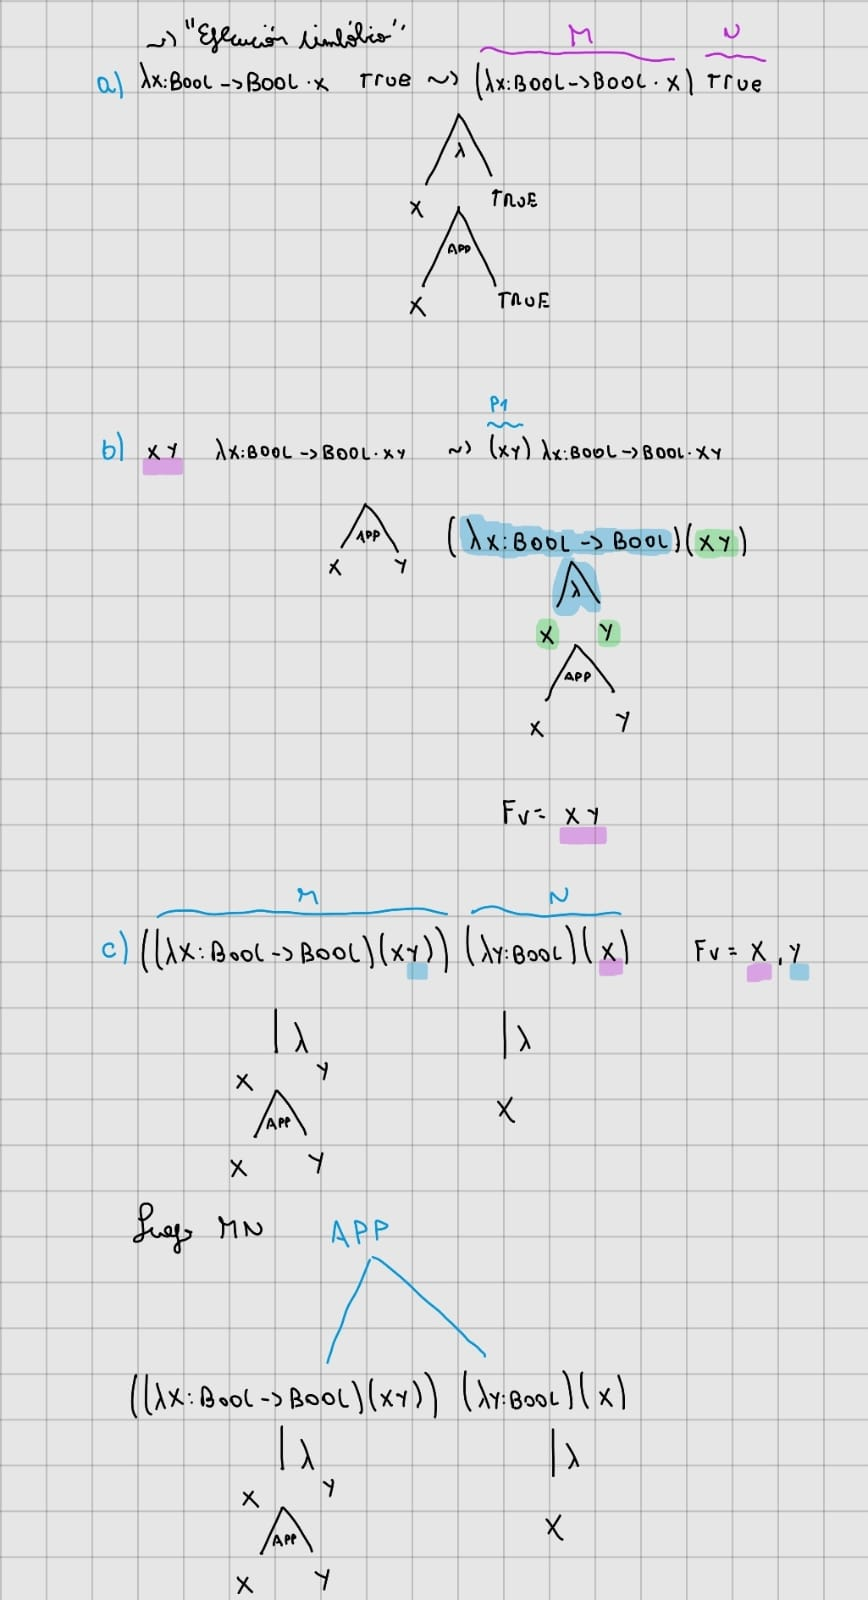
\includegraphics[width=\linewidth]{assets/arbol_sintatico.jpg}
\end{minipage}\] 
La idea es ir aplicando como Haskell la asociación, separar en varios pasos la ejecución y luego aplicarlo. 
\end{document} 
